%%%%%%%%%%%%%%%%%%%%%%%%%%%%%%%%%%%%%%%%%%
% labInstructions.cls provides all the styles needed
% us the option 'full' to show the solutions and
% additional assistant informations
%%%%%%%%%%%%%%%%%%%%%%%%%%%%%%%%%%%%%%%%%%
\documentclass[]{labInstructions}

\usepackage{siunitx}

\ifthenelse{\boolean{showAdditional}}{
\title{{\Huge \scshape Laboratoire de physique des particules}\\\vspace{0.5cm}{\Large Laboratoire PHYS-F-311 -- \textit{Version Assistants}}}}
{\title{{\Huge \scshape Laboratoire de physique des particules}\\\vspace{0.5cm}{\Large Laboratoire PHYS-F-311}}}

\author{~}
\date{~}

\begin{document}

\maketitle
\thispagestyle{empty}
\setcounter{tocdepth}{2}
\setlength{\parskip}{2pt}
\tableofcontents
\setlength{\parskip}{8pt}
\setcounter{page}{1}
\vspace{3cm}
\ifthenelse{\boolean{showAdditional}}{
\begin{additional}
\textbf{Attention!}\\
Cette version contient des informations supplémentaires destinées aux assistants. Celles-ci sont indiquées par une barre grise située sur le côté gauche.
\end{additional}
}

%%%%%%%%%%%%%%%%%%%%%%%%%%%%%%%%%%%%%%%%%%
% Introduction
%%%%%%%%%%%%%%%%%%%%%%%%%%%%%%%%%%%%%%%%%%
\section{Introduction}

Cette manipulation a pour but la caract\'erisation d'un module optique (OM) développé pour l'expérience AMANDA. Afin d'étidier les propriétés de cet OM, vous devrez mettre au point le dispositif nécéssaire à la prise de mesure. Après avoir pris connaissance avec le dispositif, vous serez ainsi amené à développer vous même la logique d'acquisition des données. Vous analyserez ensuite celle-ci grâce au outils statistiques et informatiques que vous aurez vous en cours. 

\pagebreak


%%%%%%%%%%%%%%%%%%%%%%%%%%%%%%%%%%%%%%%%%%
% Common description of the materials
%%%%%%%%%%%%%%%%%%%%%%%%%%%%%%%%%%%%%%%%%%
\section{Le matériel expérimental}

\subsection{Scintillateurs}

\subsection{Photo-multiplicateurs}

\begin{figure}
    \centering
	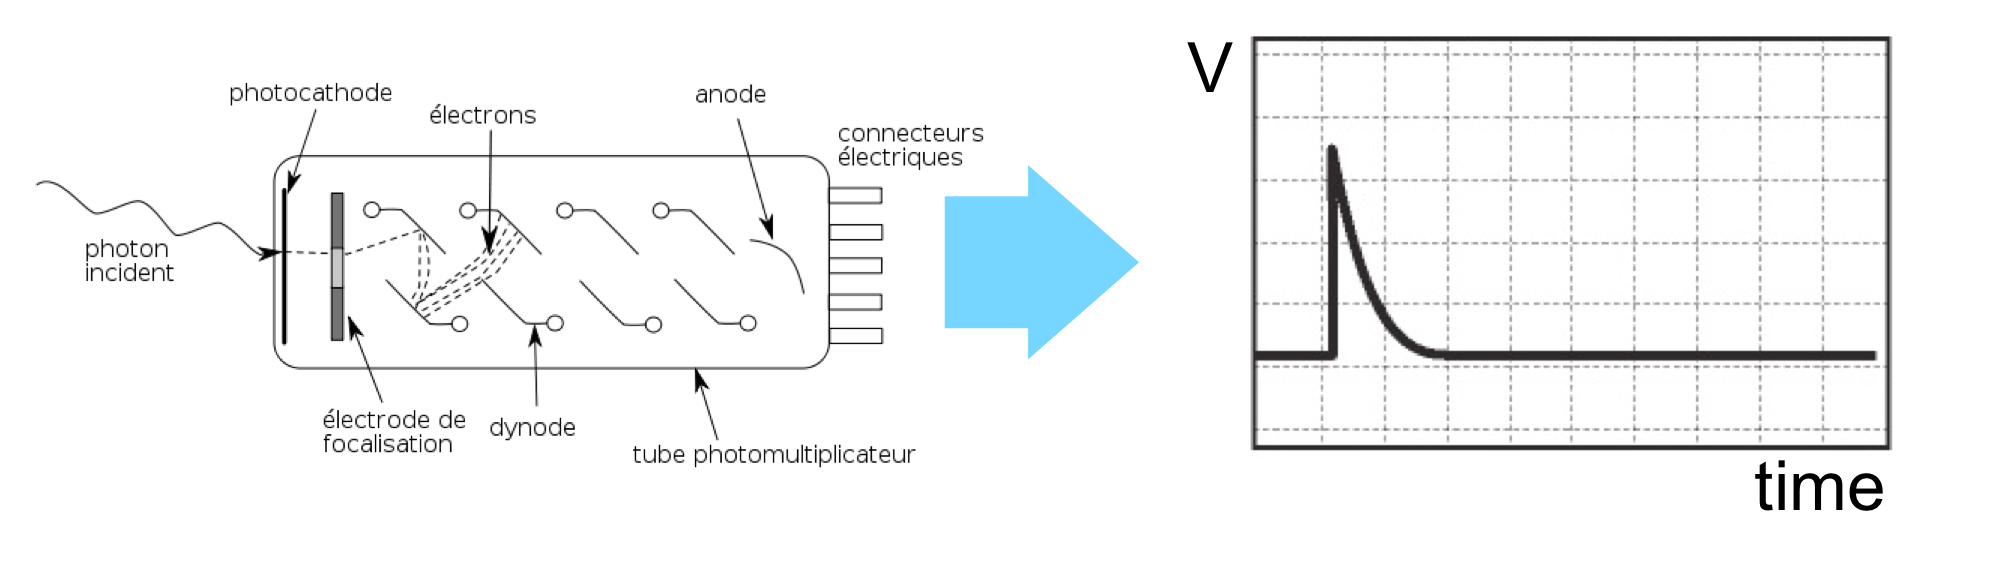
\includegraphics[width=\textwidth]{figures/PMT_readout.png}
    \caption{Schema du fonctionnement d'un photo-multiplicateur(PMT).}
    \label{fig:PMT_readout} 
\end{figure}

Nous allons à présent étudier les différentes composantes d'un spectre en charge typique de la réponse d'un photo-multiplicateur.\\

\begin{figure}[!h]
    \center{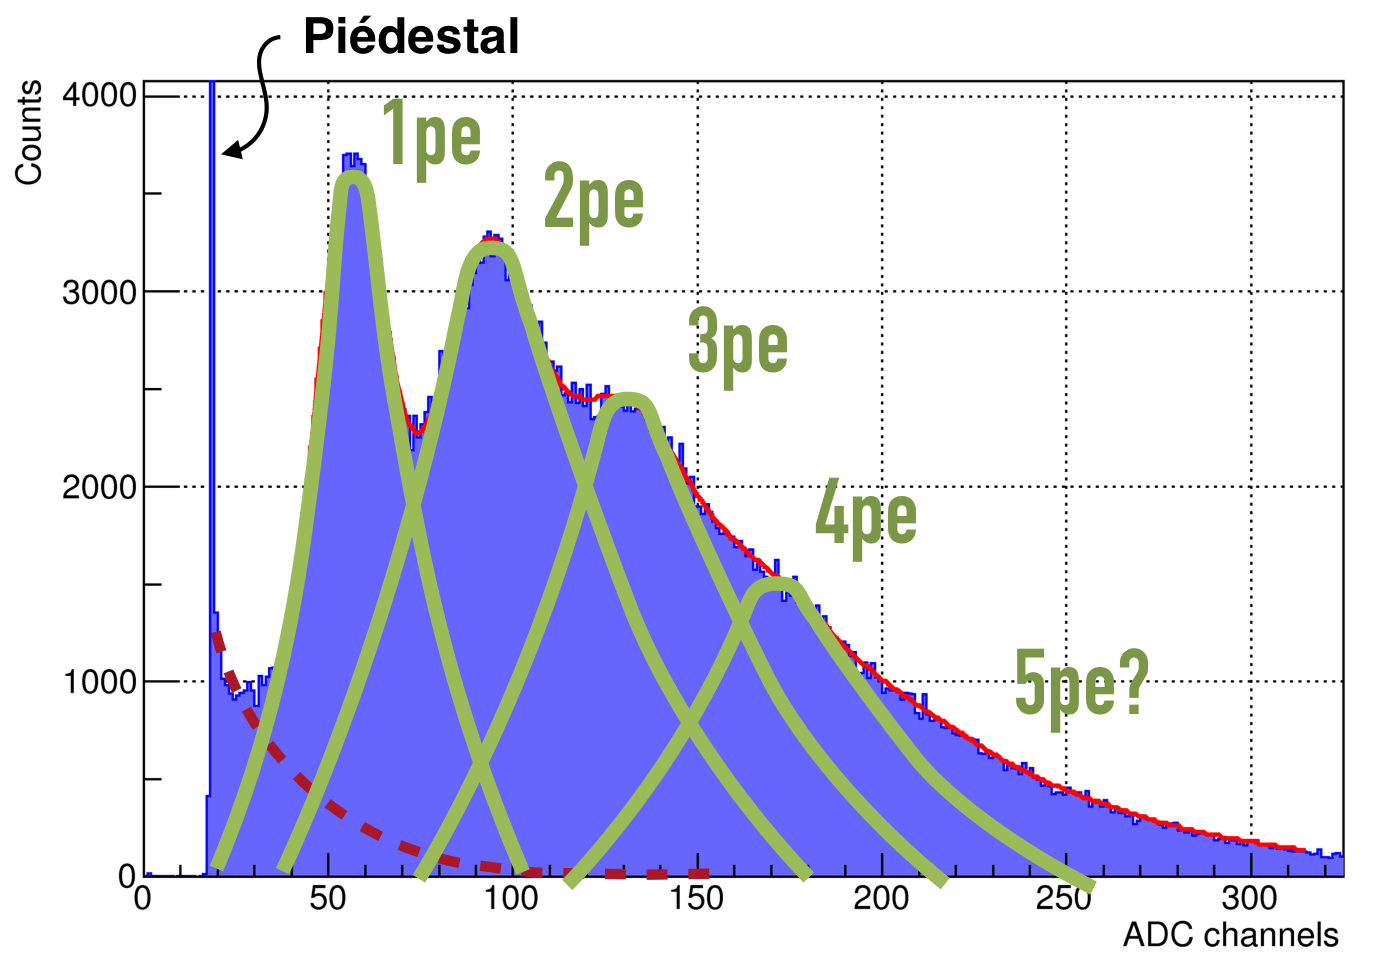
\includegraphics[width=0.7\textwidth]
    {figures/SpectreEnCharge.png}}
    \caption{\label{fig:spectre} Spectre en charge d'un photo-multiplicateur.}
\end{figure}

\textbf{Piédestal :} Il s'agit d'évènements sans charge qui prennent la forme d'un pic en zéro. Afin de se débarrasser de cet effet, il vous faudra régler au mieux votre seuil.\\

\textbf{Dark current :} Il s'agit de bruit associé au PM, il survient lorsqu'un électron est arraché à une dynode sans qu'un photon incident n'arrive à la photo-cathode. Il nous donne une exponentielle décroissante. Cet effet est exacerbé lorsque la tension aux bornes du photo-multiplicateur est élevée. \\

\textbf{Pic des photo-électrons :} Ce sont le réponse en charge du PM pour différent nombre de photo-électrons.\\

Le largeur de la gaussienne du premier photo-électron (1pe) va nous donner la résolution en charge du PM. La relation entre la hauteur des gaussiennes nous est donné par la distribution de Poisson.

\subsection{Aquisition de donn{\'e}es}

\begin{figure}
    \centering
    \begin{subfigure}[t]{0.2\textwidth}
        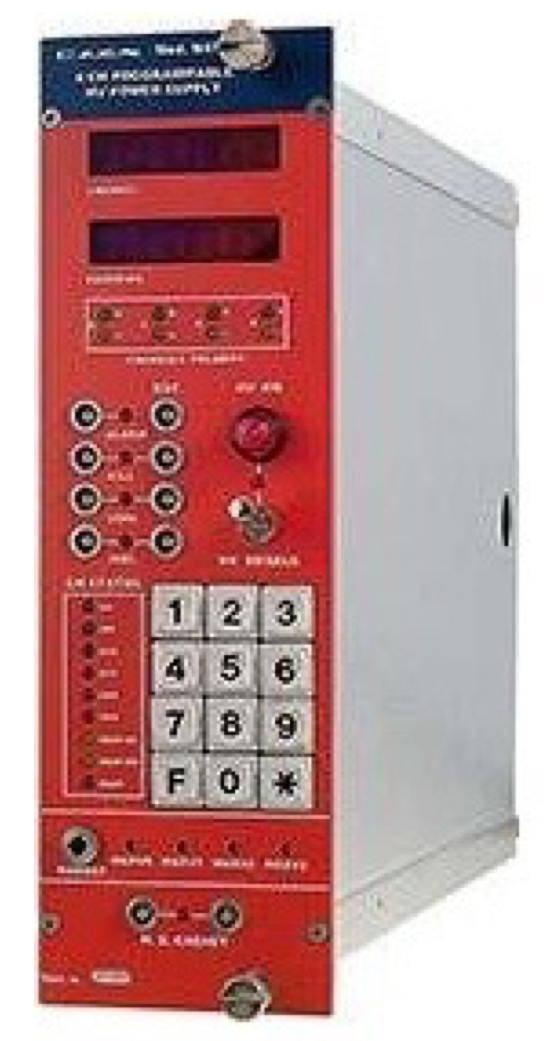
\includegraphics[height=0.25\textheight, width=\textwidth, keepaspectratio]{figures/Alim1.png}
        \caption{Alimentation de haute tension}
        \label{fig:HV1}
    \end{subfigure}
    \hfill
    \begin{subfigure}[t]{0.2\textwidth}
        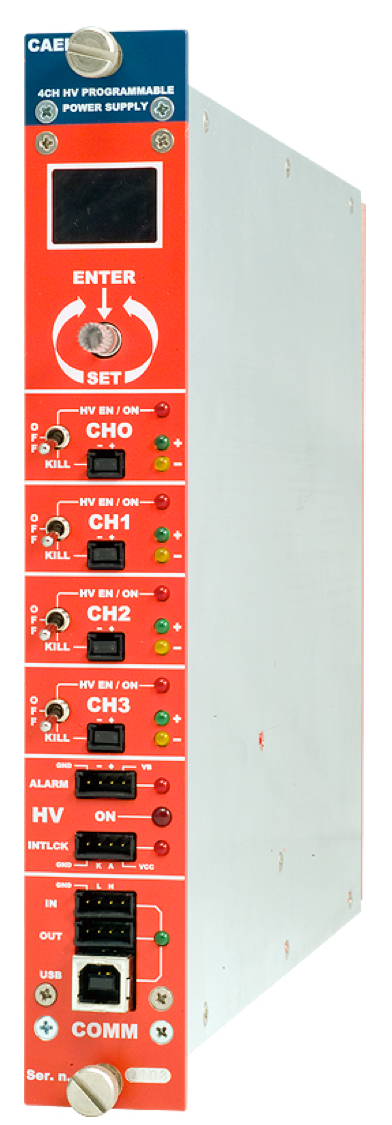
\includegraphics[height=0.25\textheight, width=\textwidth, keepaspectratio]{figures/Alim2.png}
        \caption{Alimentation de haute tension}
        \label{fig:HV2}
    \end{subfigure}
    \hfill
    \begin{subfigure}[t]{0.2\textwidth}
        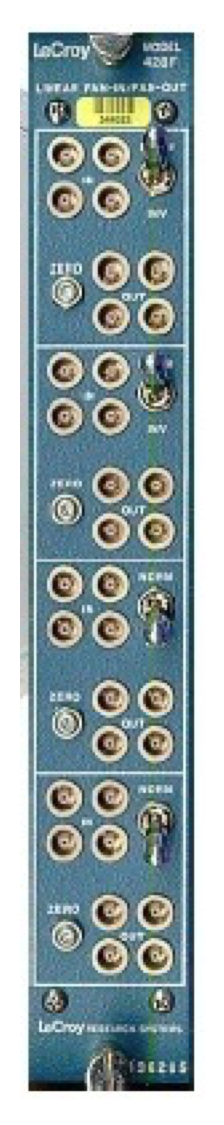
\includegraphics[height=0.25\textheight, width=\textwidth, keepaspectratio]{figures/FanInFanOut.png}
        \caption{Distributeur de signal \emph{fan-in-fan-out}}
        \label{fig:fifo}
    \end{subfigure}
    \hfill
    \begin{subfigure}[t]{0.2\textwidth}
        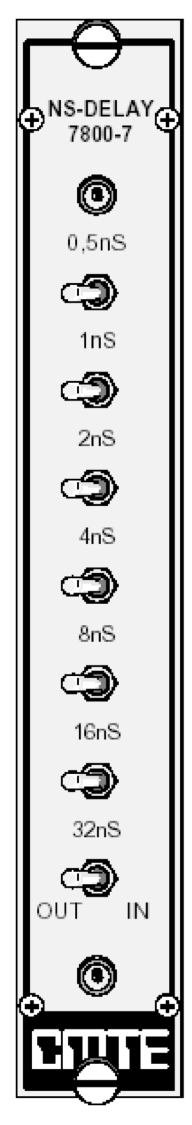
\includegraphics[height=0.25\textheight, width=\textwidth, keepaspectratio]{figures/delay.png}
        \caption{Delayeur de signal}
        \label{fig:delay}
    \end{subfigure}
    
	\vspace{1cm}
    \begin{subfigure}[t]{0.2\textwidth}
        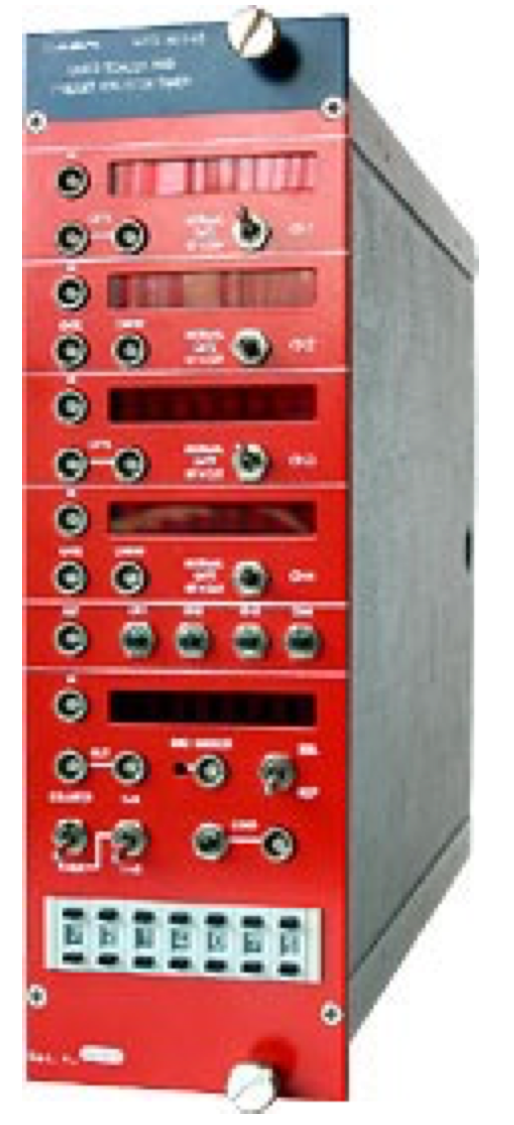
\includegraphics[height=0.25\textheight, width=\textwidth, keepaspectratio]{figures/scaler.png}
        \caption{Scaler NIM}
        \label{fig:scaler1}
    \end{subfigure}
    \hfill
    \begin{subfigure}[t]{0.25\textwidth}
        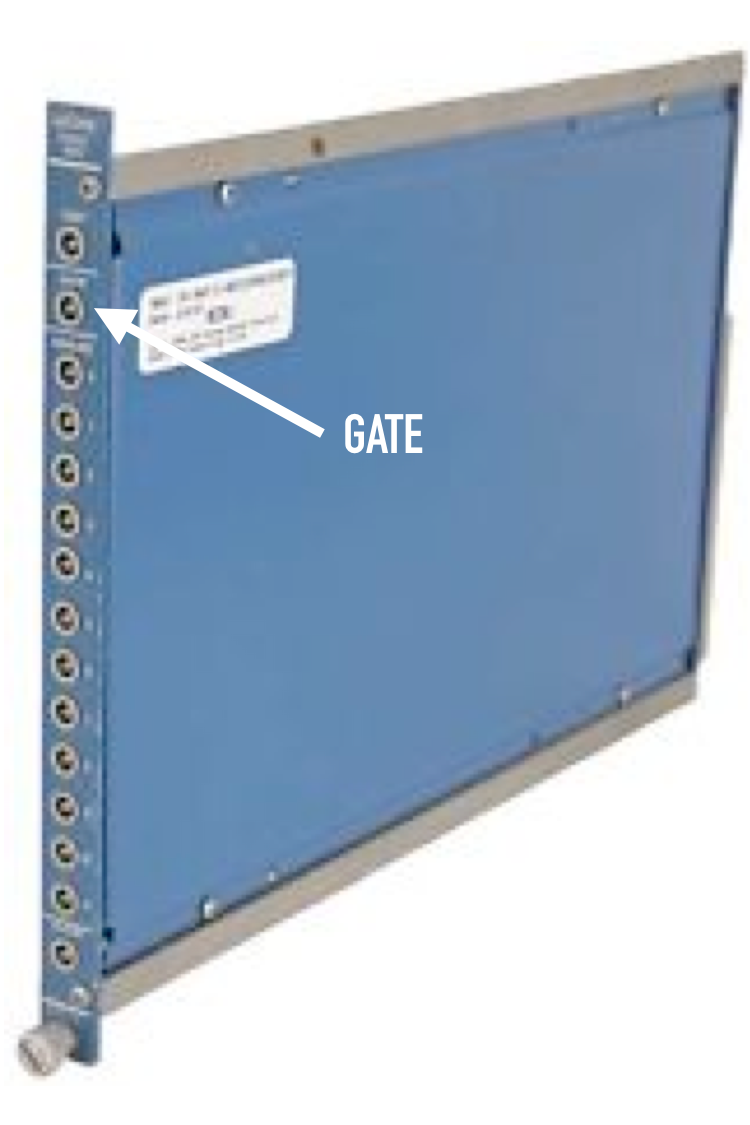
\includegraphics[height=0.25\textheight, width=\textwidth, keepaspectratio]{figures/gate.png}
        \caption{Scaler CAMAC}
        \label{fig:scaler2}
    \end{subfigure}    
    \hfill
    \begin{subfigure}[t]{0.45\textwidth}
        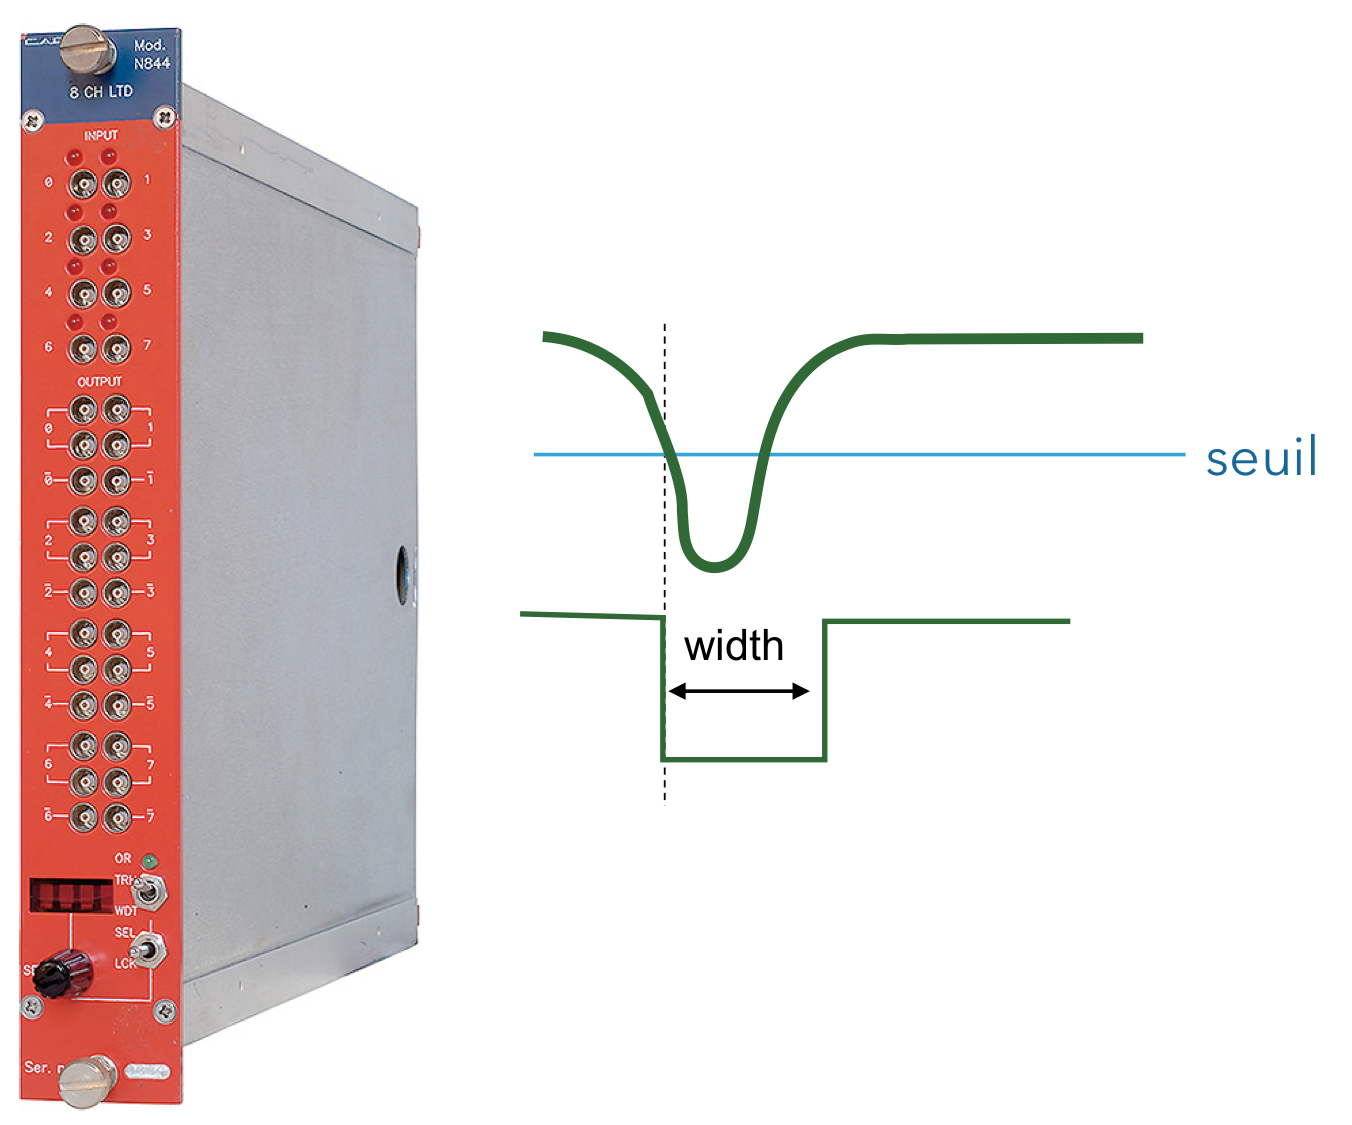
\includegraphics[height=0.3\textheight, width=\textwidth, keepaspectratio]{figures/Discriminateur.png}
        \caption{Discriminateur}
        \label{fig:discriminator}
    \end{subfigure}

	\vspace{1cm}    
    \begin{subfigure}[t]{0.45\textwidth}
        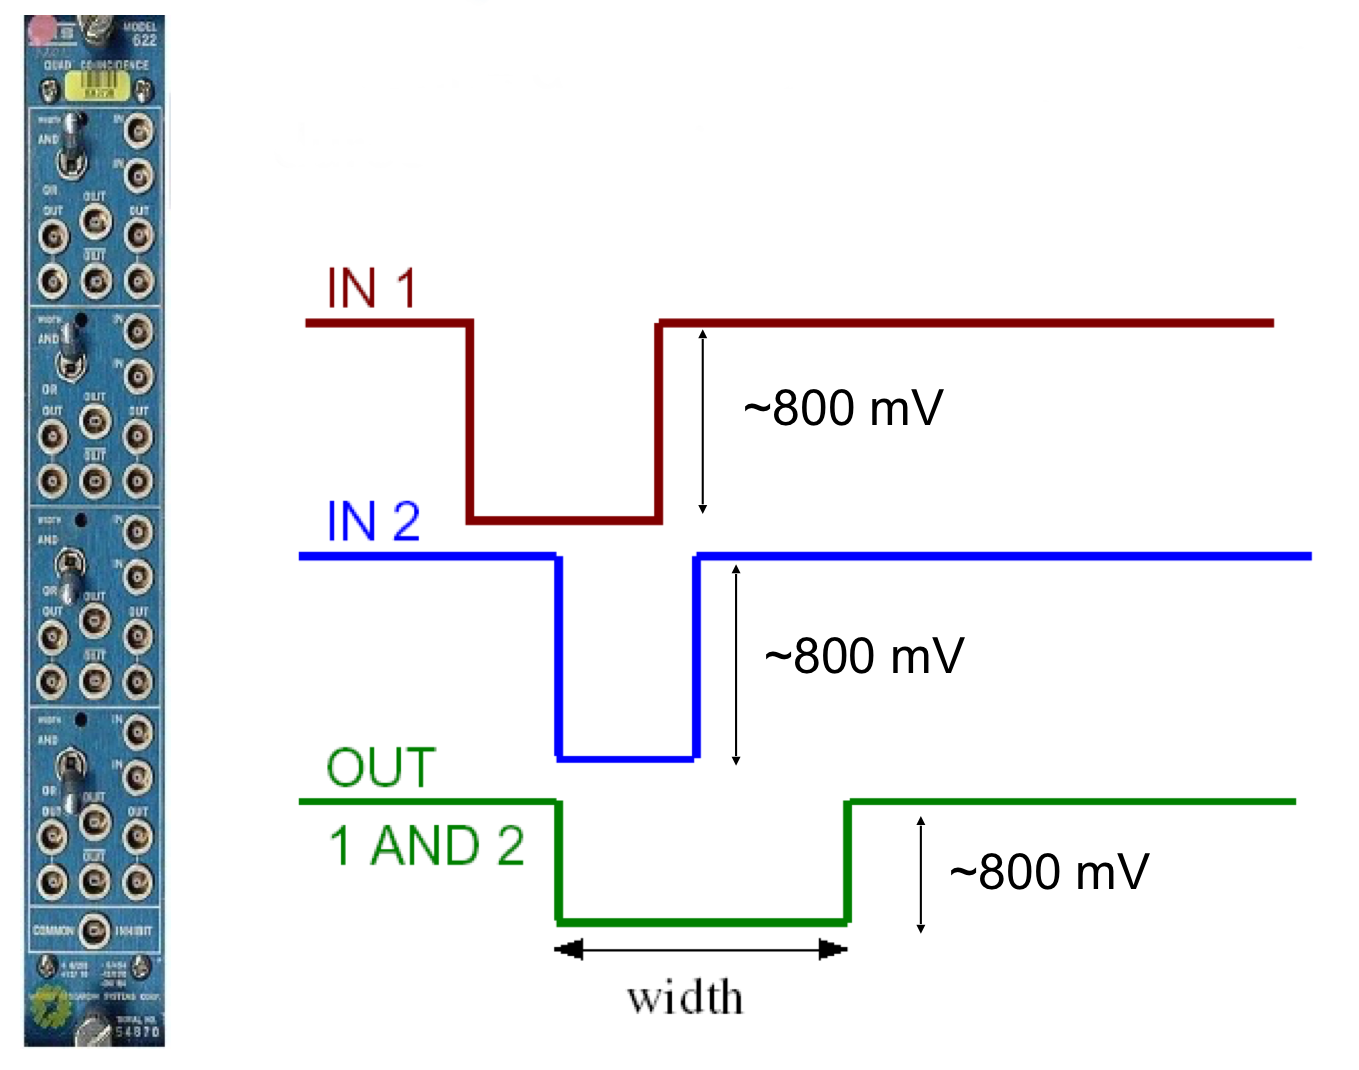
\includegraphics[height=0.3\textheight, width=\textwidth, keepaspectratio]{figures/UniteDeCoincidence_crop.png}
        \caption{Unit{\'e} de co{\"i}ncidence}
        \label{fig:coincidence}
    \end{subfigure}
    \hfill
    \begin{subfigure}[t]{0.45\textwidth}
        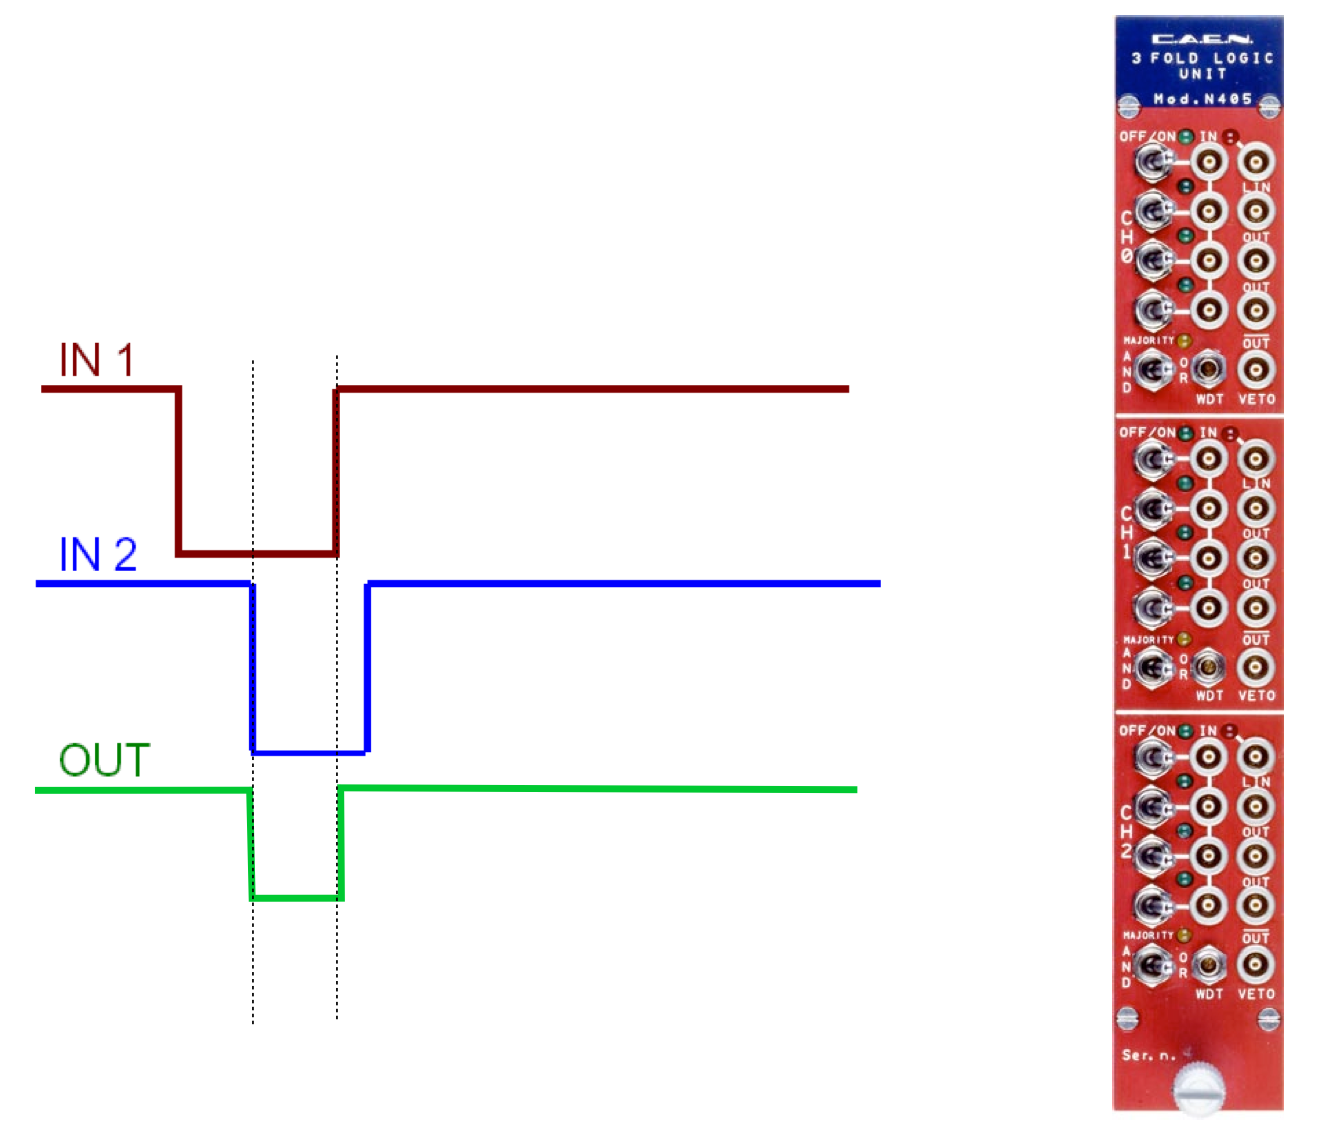
\includegraphics[height=0.3\textheight, width=\textwidth, keepaspectratio]{figures/UniteLogiqueProgrammable.png}
        \caption{Unit{\'e} logique programmable}
        \label{fig:plu}
    \end{subfigure}
    \caption{Appareils utilis{\'e}s dans les dispositifs.}
    \label{fig:devices}
\end{figure}

%%%%%%%%%%%%%%%%%%%%%%%%%%%%%%%%%%%%%%%%%%
% Brief intro to statistics
%%%%%%%%%%%%%%%%%%%%%%%%%%%%%%%%%%%%%%%%%%
\section{Methodes d'analyse statistique}

Au cours de ce laboratoire, il vous faudra analyser les données que vous aurez recueillies. Pour cela, vous aurez à votre disposition plusieurs iPython Notebook que vous étudierez en profondeur lors du cours de statistique. Ces différents outils sont accessibles via le lien suivant:\\
\url{https://github.com/zemrude/PHYS-F-311}

\subsection{Méthode Monte Carlo}
Afin de développer votre méthode d'ajustement, il vous sera demandé, dans un premier temps,  de créer un ensemble de données que vous générerez via la technique de simulation Monte Carlo (MC). Vous avez à votre disposition deux méthodes pour générer vos données: la transformation inverse et le "Hit and Miss". A l'aide de ces deux techniques, vous serez en mesure de générer des évènements aléatoire suivant la distribution de votre choix (gaussienne, loi exponentielle, ...).

\subsubsection{Hit $\&$ Miss}
La méthode Hit $\&$ Miss ou méthode du rejet consiste à générer aléatoirement un grand nombre d'évènements et à ne sélectionner ensuite que ceux remplissant les conditions pré-établies, i.e. les évènements sous la courbe de la distribution choisie. 

\begin{figure}[h!]
\center{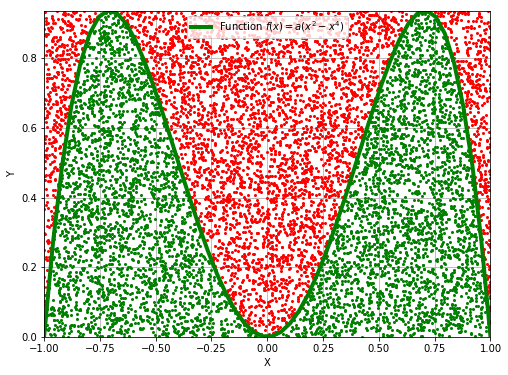
\includegraphics[width=0.6\textwidth]{figures/Hit_and_miss.png}}
\caption{Simulation obtenue par la méthode du Hit $\&$ Miss. Les points représentent les évènements générés aléatoirement. Les éléments en vert sont ceux qui ont remplissent la condition fixée pour suivre la distribution souhaitée. Les points rouges sont rejetés et auront donc été simulés en vain.}
\label{fig:HitMiss}
\end{figure}

Pour notre exemple illustré par la figure \ref{fig:Inverse}, la fonction $f(x)=a(x^{2}-x^{4})$ a été choisie. La figure \ref{fig:HitMiss} illustre la méthode du Hit $\&$ Miss en indiquant en vert les points qui sont sous la courbe de la distribution que l'on souhaite reproduire. Les points rouges seront rejetés. Cette méthode demande donc plus de ressources afin d'obtenir suffisamment de statistique puisqu'une partie des évènements générés ne  sera finalement pas utilisée.

\subsubsection{Transformation inverse}
A l'aide de cette méthode,  un échantillon aléatoire de nombres suivant une distribution donnée peut être directement produit. Les données aléatoires sont obtenues à partir de l'inverse de la fonction de répartition. Cette méthode se base sur le théorème de la réciproque. Dans un premier temps, il nous faut calculer l'inverse de notre fonction, $F(x)$, en fonction de $x$. Les évènements générés aléatoirement seront ensuite passé dans la fonction inverse afin d'obtenir la distribution souhaitée. 

\begin{figure}[h!]
\center{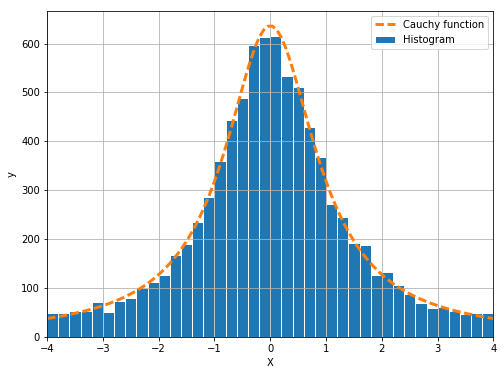
\includegraphics[width=0.6\linewidth]{figures/Inverse_transformation.png}}
\caption{Histogramme des évènements générés par la méthode de transformation inverse pour la distribution de Cauchy.}
\label{fig:Inverse}
\end{figure}

Pour notre exemple illustré par le graphique \ref{fig:Inverse}, nous allons considérer la loi de Cauchy, dont la fonction de répartition s'écrit:

\begin{equation}
F(x) = \frac{1}{2} + \frac{1}{\pi} \arctan \left(\frac{x - x_{0}}{a}\right) \, .
\end{equation}

On a alors:

\begin{equation}
u = F(x) \Longleftrightarrow x = x_{0} + a \tan \left[ \pi  \left(u - \frac{1}{2} \right)  \right] \, .
\end{equation}

La simulation peut donc être obtenue en suivant :

\begin{equation}
X = x_{0} + a \tan \left[ \pi  \left(U - \frac{1}{2} \right)  \right] \, .
\end{equation}

La fonction de Cauchy est indiquée en orange alors que les données simulées obtenues à partir de notre méthode inverse sont mise en histogramme. On peut voir que la distribution de ces évènements reproduit correctement la loi de Cauchy.

\subsection{Ajustement}
Nous allons à présent développer la méthode d'ajustement sur les données que vous venez d'obtenir par la méthode Monte Carlo de votre choix. Deux méthodes vous sont à nouveau proposées pour ce "fit": la méthode des moindre carré ($\chi^2$) et la méthode du maximum de vraisemblance. Ces deux méthodes permettent de comparer nos données avec les prédictions théorique de notre modèle. Une fois au point, vous pourrez donc utiliser cet ajustement sur vos données réelles afin de confirmer que votre échantillon a bien le comportement attendu. 

\textbf{Remarque :} La minimisation n'est pas effectuée directement sur les données mais sur les données déjà représentées en histogramme.

\subsubsection{Moindre carré - $\chi^{2}$}
Considérons la distribution de nos évènements générés par MC  que l'on désire ajuster au mieux par une fonction $f(x)$ que nous choisirons de façon pertinente en fonction du phénomène étudier. Nous cherchons les paramètres de cette fonction minimisant la somme des carrés des distances entre la hauteur de nos barres d'histogrammes, $y_i$, en $x_i$ et $f(x_i)$, autrement dit:

\begin{equation}
\chi^2 = \sum_{i=1}^{N} \left[ y_i - f(x_i) \right]^2 \, .
\end{equation}

Pour notre exemple, nous considérons une distribution d'évènement suivant une décroissance exponentielle dont nous tentons de trouver le temps de vie, $\tau$. Notre fonction est donc donnée par:

\begin{equation}
f(x) = \alpha \exp(-x / \tau) \, .
\end{equation}

La valeur de $\tau$ minimisant $\chi^2$ est illustrée par la figure \ref{fig:chi2}. Celle-ci est utilisée pour l'ajustement de la figure de droite.

\begin{figure*}[h!]
    \centering
    \begin{minipage}[b]{0.48\linewidth}
    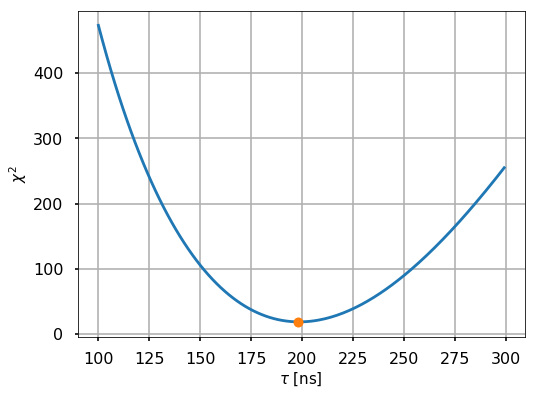
\includegraphics[width=\linewidth]{figures/chi_2.png}
    \end{minipage}
    \hfill
    \begin{minipage}[b]{0.51\linewidth}
    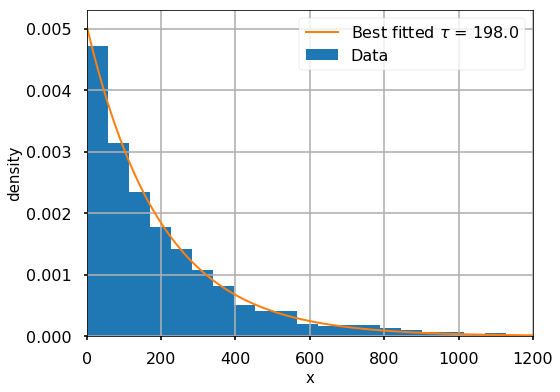
\includegraphics[width=\linewidth]{figures/chi_2_bestfit.png}
    \end{minipage}
    \caption{\textbf{Gauche :} La valeur de $\tau$ minimisant $\chi^2$ est désignée par le point orange. \textbf{Droite :} Le fit obtenu à partir de $\tau_{best}$ (orange) est mis en graphique au côté de la distribution des données MC que nous tentions d'ajuster.}
    \label{fig:chi2}
\end{figure*}

\subsubsection{Maximum de vraisemblance}
La méthode de maximum de vraisemblance est une méthode statistique nous permettant d'évaluer la valeur la plus "vraisemblable" des paramètres d'un modèle probabiliste. 

Pour notre exemple, nous considérons la loi normale exprimée comme suit:

\begin{equation}
f(x) = \frac{1}{\sigma\sqrt{2\pi}} \exp{-\frac{1}{2} \left( \frac{x-\mu}{\sigma}\right)^2} \,  , 
\end{equation}

où $\sigma$ est l'écart type et $\mu$ est la moyenne. Nous allons à présent tenter de trouver la valeur de $\mu$ optimisant la fonction de vraisemblance,  $\mathcal{L}$. Pour cela nous fixons l'écart type de la Gaussienne et laissons varier la moyenne. Nous trouvons ensuite la valeur de $\mu$ qui minimise $-\log{\mathcal{L}}$, comme illustré par la figure \ref{fig:MaxLikelihood}.

\begin{figure*}[h!]
    \centering
    \begin{minipage}[b]{0.49\linewidth}
    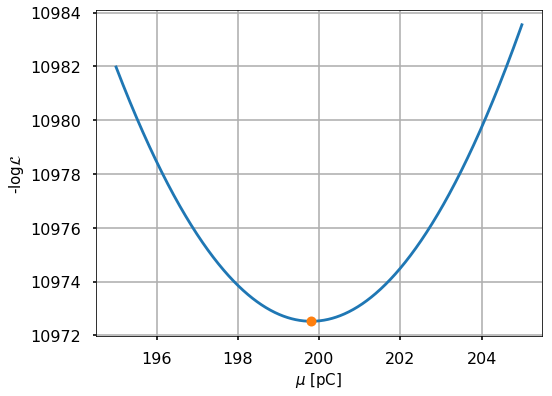
\includegraphics[width=\linewidth]{figures/MaxLikelihood.png}
    \end{minipage}
    \hfill
    \begin{minipage}[b]{0.49\linewidth}
    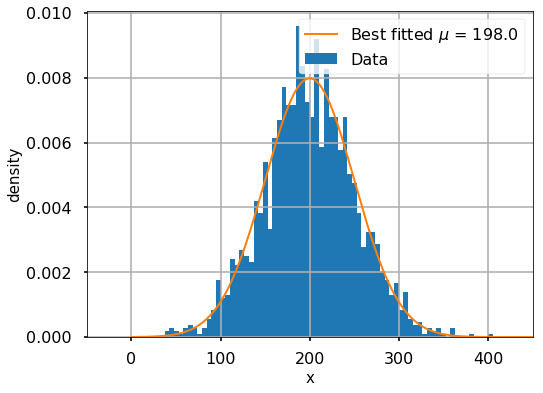
\includegraphics[width=\linewidth]{figures/MaxLikelihood_bestFit.png}
    \end{minipage}
    \caption{\textbf{Gauche :} La valeur de $\mu$ minimisant $-\log{\mathcal{L}}$ est désignée par le point orange. \textbf{Droite :} Le fit obtenu à partir de $\mu_{best}$ (orange) est mis en graphique au côté de la distribution des données MC que nous tentions d'ajuster.}
    \label{fig:MaxLikelihood}
\end{figure*}


\subsection{Erreur sur l'ajustement}
Nous pouvons également estimer l'erreur associée à une valeur ajustée. Nous allons pour cela faire varier de l'unité choisie (1, 2, 3, ...) la valeur minimale de la méthode choisie. Nous obtiendrons ainsi l'erreur en terme de $\sigma$. L'erreur sur le paramètre à ajuster nous indique alors dans quelle mesure ce paramètre varierait si on répétait le processus de minimisation plusieurs fois.

Pour notre exemple, nous nous intéresseront à la méthode de maximum de vraisemblance. Nous ferons donc varier d'une unité la valeur minimale de  $-\log{\mathcal{L}}$. La barre noire sur le graphique \ref{fig:error} indique l'erreur sur $\mu$ ainsi obtenue.


\begin{figure}[h!]
\center{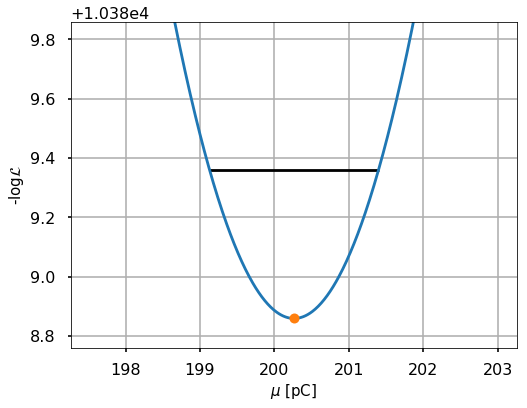
\includegraphics[width=0.6\linewidth]{figures/error.png}}
\caption{Erreur de $1\sigma$ obtenue pour l'exemple précédent de l'ajustement selon la méthode du maximum de vraisemblance.}
\label{fig:error}
\end{figure}






%%%%%%%%%%%%%%%%%%%%%%%%%%%%%%%%%%%%%%%%%%
% Description of the Experiments
%%%%%%%%%%%%%%%%%%%%%%%%%%%%%%%%%%%%%%%%%%

\section{Dispositif: Effet Tcherenkov par des électrons}

Cette manipulation a pour but la caractérisation d'un module optique (OM) développé pour l'expérience AMANDA. Afin d'étudier les propriétés de cet OM, vous devrez mettre au point le dispositif nécessaire à la prise de mesure. Après avoir pris connaissance avec le dispositif, vous serez ainsi amené à développer vous même la logique d'acquisition des données. Vous analyserez ensuite celles-ci grâce aux outils statistiques et informatiques que vous aurez vu en cours. \\

Cette manipulation utilise une source de radiation $\beta^+$ composée de Strontium $^{90}$Sr. Les électrons émis par la source traverse ensuite une plaque de quartz d'indice de réfraction  $n = 1.478$. Lors de leur passage, les électrons vont produire un rayonnement Tcherenkov qui pourra être détecté par l'OM. Dans ce dispositif, l'OM se trouve à une position fixe située à un angle de 45$^{\circ}$ par rapport à la direction d'émission des électrons. La source radioactive est combinée à un spectromètre qui va nous permettre de sélectionner l'énergie cinétique des électrons afin de récolter un maximum de rayonnement Tcherenkov dans l'OM. Pour déterminer l'intensité du courant à fournir au spectromètre pour obtenir des électrons de cette énergie, vous devrez d'abord résoudre l'exercice 2.\\

Une fois cette valeur trouvée, vous pouvez allumer le spectromètre. Celui-ci est calibré sur la partie descendante de la courbe d'hystérèse, il vous faudra donc respecter les conditions d'utilisation décrites ci-dessous.\\

\textbf{Mode d'emploi du spectromètre :}
\begin{quote}
    \begin{itemize}
        \item Démarrez à $I$ = 0 A
        \item Aller à saturation $I$ $\sim$ 2,6 A
        \item Descendre à la valeur $I_t$ désirée
    \end{itemize}
\end{quote}
\textbf{Remarque :} Si on veut changer $I_t$ pour une valeur plus petite, on descend vers cette valeur. En revanche, si on veut augmenter cette valeur, on doit recommencer le cycle d'hystérèse. 

\begin{figure}[!h]
    \centering
    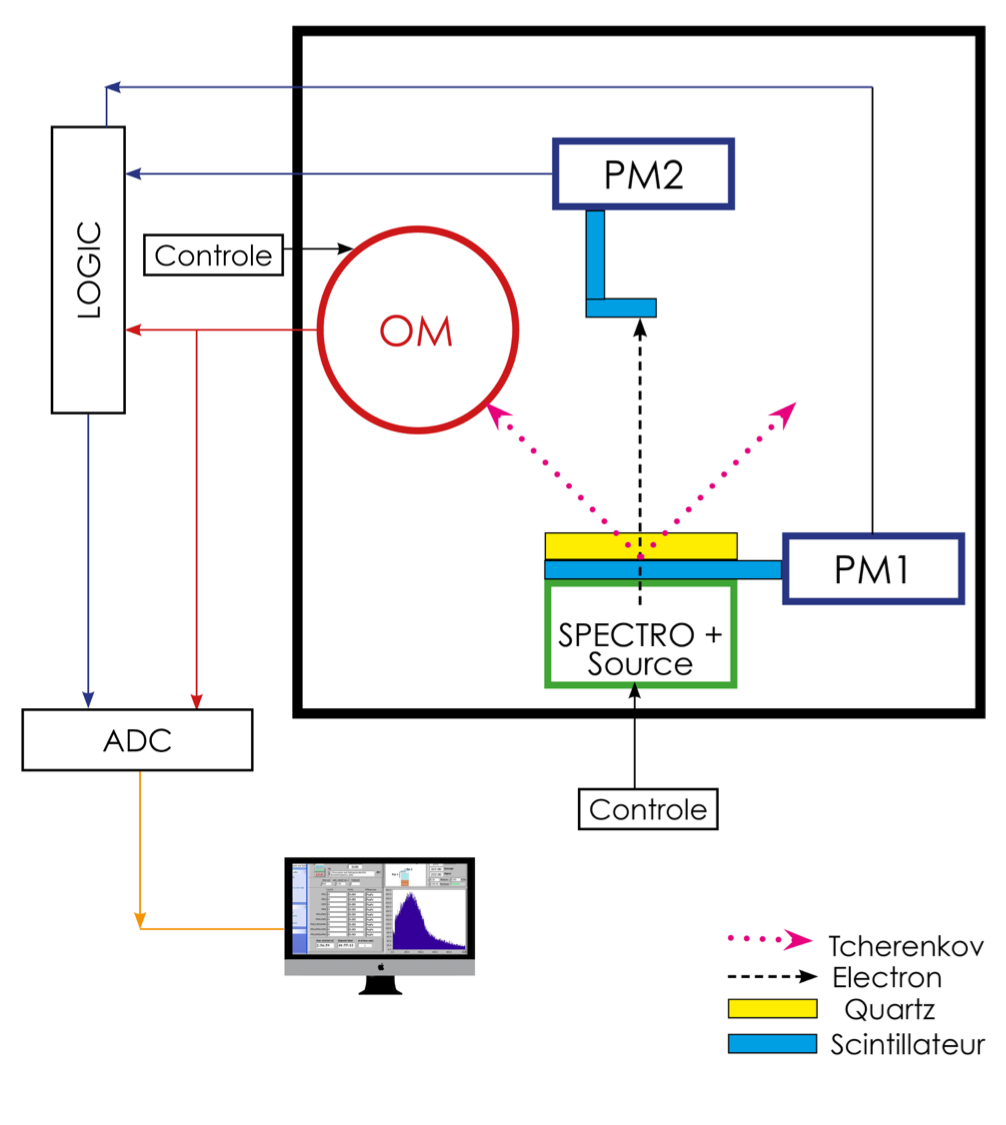
\includegraphics[width=0.5\textwidth]{figures/Dispositif_1.png}
    \caption{Dispositif expérimental de l'effet Tcherenkov produit par des électrons.}
    \label{fig:dispo1} 
\end{figure}

Dans ce dispositif, sont également présent 2 photo-multiplicateurs (PMs) chacun relié à un scintillateur. Le premier (PM1) est situé entre la source et la plaque de quartz et nous permet de vérifier qu'un électron a été émis par la source. Le second PM confirme que l'électron a bien traversé le quartz. Ces PMs ont donc pour but d'assurer que le signal détecté par l'OM est en coïncidence avec un électron qui a produit des photons Tcherenkov.


\subsection{Exercices Préparatoires}

\subsubsection{Exercice 1}
Sachant que l'OM est placé à un angle de $45^\circ$ par rapport à la direction d'émission des électrons ($m_\mathrm{e} = 0.511$\,MeV/$c^2$) de la source de strontium, à quel courant faut-il régler le spectromètre pour récolter un maximum de rayonnement Tcherenkov dans l'OM, sachant que l'indice de réfraction du quartz est de $1.478$?\\

Le graphique suivant vous donne la relation entre l'énergie cinétique des électrons et l'intensité du courant.

\begin{figure}[!h]
    \center{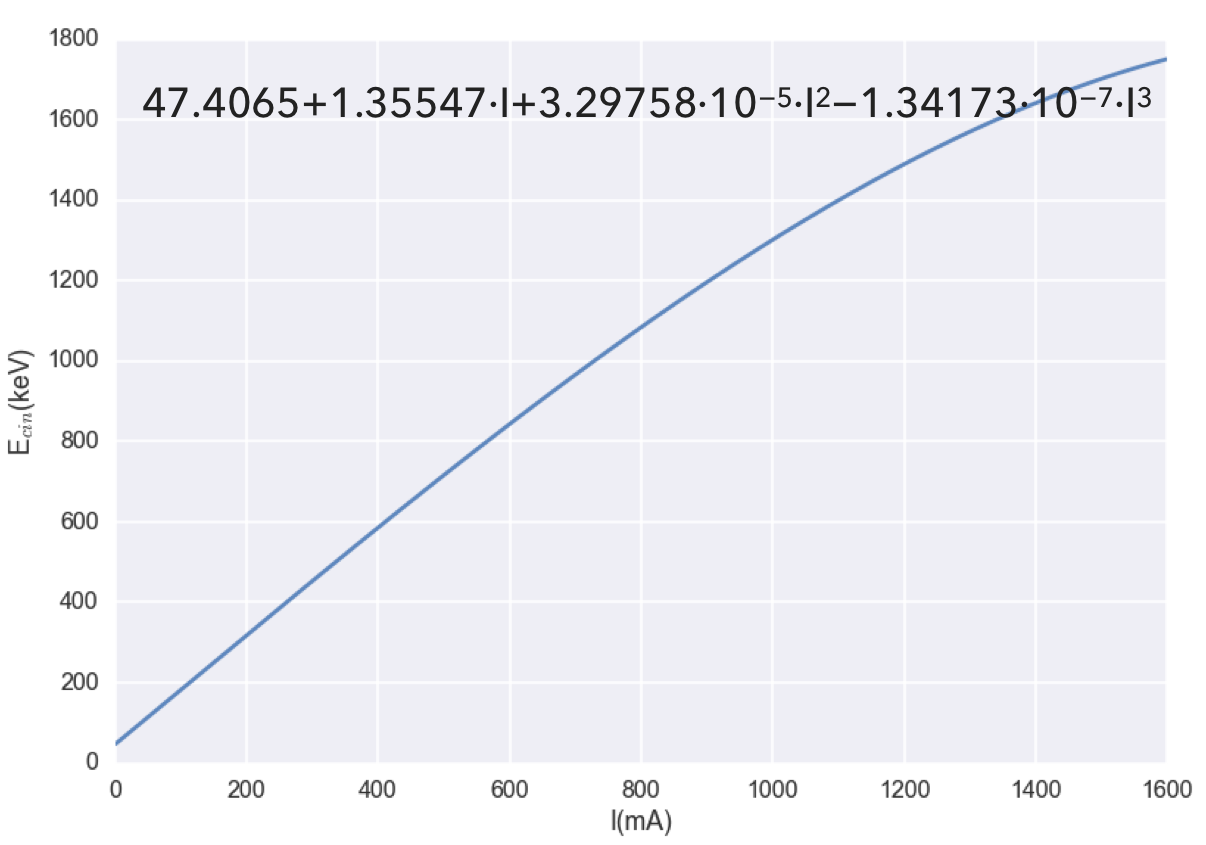
\includegraphics[width=0.5\textwidth]
    {figures/Relation_Ecin_I.png}}
    \caption{\label{fig:spectro} Relation entre l'intensité du courant fourni au spectromètre et l'énergie cinétique des électrons.}
\end{figure}

\ifthenelse{\boolean{showAdditional}}{
\begin{additional}
\begin{align*}
\beta &= \frac{1}{n\cos\Theta_\mathrm{c}} = 0.9568\\
 &= \frac{pc}{E}\\
 &= \frac{\sqrt{E^2-m_\mathrm{e}^2c^4}}{E}\\
 &\\
E &= \sqrt{\frac{m_\mathrm{e}^2c^4}{1 - \beta^2}} = 1.7575\,\mathrm{MeV}\\
E_\mathrm{cin}&=E- m_\mathrm{e}\\
 &= 1.247\,\mathrm{MeV} \\
&\Rightarrow \boxed{I \approx 950\,\mathrm{mA}} \\
\end{align*}
\end{additional}
}

\subsubsection{Exercice 2}
Calculer l'ordre de grandeur du nombre de photons émis entre $350$ et $500$\,nm par un électron de $1247$\,keV d'énergie cinétique traversant une fenêtre de quartz de 1\,mm d'épaisseur, sachant que pour ce domaine de longueurs d’onde, l'indice de réfraction du quartz varie de moins de 1\% et peut être considéré constant ($1.478$). Négliger la perte d'énergie de l'électron dans le quartz.\\ $\alpha = 1/137$

\ifthenelse{\boolean{showAdditional}}{
\begin{additional}
Formule de \emph{Frank-Tamm}:
\begin{align*}
\frac{\mathrm{d}N}{\mathrm{d}x} &= \int_{\lambda_0}^{\lambda_1} \frac{2\pi\alpha z^2}{\lambda^2} \sin^2\Theta_\mathrm{c} \mathrm{d}\lambda\\
&=\frac{\pi}{137}\int_{350\,\mathrm{nm}}^{500\,\mathrm{nm}}\frac{\mathrm{d}\lambda}{\lambda^2}\\
N&=\frac{\pi}{137}\cdot\left(\frac{1}{350\,\mathrm{nm}}-\frac{1}{500\,\mathrm{nm}}\right)\cdot1\,\mathrm{mm}\\
&=\boxed{19.65}
\end{align*}
\end{additional}
}

\subsubsection{Exercice 3}
En supposant que le diamètre du collimateur placé devant la photocathode de l'OM est de 6 cm et qu'il se trouve à 17\,cm de la fenêtre de quartz, combien de photoelectrons l'OM peut-il enregistrer par électron de la source, en supposant une transmittance $T$ de 90\% et sachant que l'efficacité quantique est de $\epsilon_\mathrm{q}=15\%$?

\ifthenelse{\boolean{showAdditional}}{
\begin{additional}
Avec $N_\mathrm{\gamma}^{\mathrm{quartz}}$ trouvé avant, on obtient:
\begin{align*}
N_{\mathrm{pe}} &= \epsilon_\mathrm{q} \cdot T \cdot N_\mathrm{\gamma}^{\mathrm{OM}}\\
 &= \epsilon_\mathrm{q} \cdot T \cdot \frac{6\,\mathrm{cm}}{2\pi \cdot 17\,\mathrm{cm} \cdot\sin\Theta_\mathrm{c}} \cdot N_\mathrm{\gamma}^{\mathrm{quartz}}\\
&= \boxed{3.58}
\end{align*}
\end{additional}
}


\subsection{Prise de mesure}

Pour cette manipulation, il vous est demandé de préparer le dispositif expérimental nécessaire à la prise de mesure. Cela implique, dans un premier temps, de :\\

\begin{center}
\fbox{
\begin{minipage}{0.75\textwidth}
\textbf{Se familiariser avec le dispositif :} 
\begin{quote}
\begin{itemize}
\item vérifier le signal des différents PMs et de l'OM
\item étudier l'efficacité des PMs
\item calibrer l'ADC
\item développer la logique d'acquisition de données
\item mesurer le bruit de fond
\end{itemize}
\end{quote}
\end{minipage}
}
\end{center}

\subsubsection{Vérification du dispositif}
Dans un premier temps, allumez votre dispositif et allumez la haute tension aux bornes des PM. Veillez ne pas changer la tension indiquée afin de ne pas endommager les PMs.\\

Après avoir calculé l'intensité du courant à fournir au spectromètre, allumer également celui-ci en suivant les instructions fournies précédement.\\

A l'aide de l'oscilloscope, vérifiez le signal provenant des différents photo-multiplicateurs (PMs) et de l'OM. Transformez ensuite votre signal analogue en signal digital à l'aide du discriminateur et observez celui-ci sur l'oscilloscope.
\subsubsection{Mesure de l'efficacité}

Il vous est ensuite demandé de mesurer l'efficacité d'un des PMs présents dans votre dispositif. Vous devrez faire cette mesure en faisant varier dans un premier temps le seuil du PM pour lequel vous mesurer l'efficacité. Une fois la valeur optimale du seuil trouvée, répétez le processus en faisant cette fois varier la tension appliquée sur le PM en question. Pour ces deux mesures, veillez également à mesurer le taux d'évènements détectés par le PM dont vous mesurez l'efficacité. Pour effectuer ces mesures, vous avez à votre disposition un scaler NIM. De quel PM allez-vous mesurer l'efficacité ?

\ifthenelse{\boolean{showAdditional}}{
\begin{additional}
\begin{itemize}
\item Mesure de l'efficacité de PM1
\item Logique : (PM1 \& PM2 \& OM) et (PM2 \& OM)
\item Mesure du rate de PM1
\end{itemize}
\end{additional}
}

\subsubsection{Calibration de l'ADC}

Nous allons à présent procéder à la calibration du convertisseur analogique-numérique (ADC ou Analogue-to-Digital Converter). En effet, l'ADC vous donne des valeurs en ADC channel, il vous faut donc connaître à quelle charge équivaut un ADC channel.\\

Pour cette calibration, il faut fournir une charge connue et constante à l'ADC. Pour cela, vous avez à votre disposition un générateur de courant continu. Comment allez-vous procéder ? 

\ifthenelse{\boolean{showAdditional}}{
\begin{additional}
\begin{itemize}
    \item Charge de l'ADC de l'ordre du pC $\to$ $Q\sim100$\,pC 
    \item Utilisation d'une résistance: $U = RI$ avec $R = 2.2$\,k$\mathrm{\Omega}$
    \item Sachant que $Q = I\mathrm{\Delta}t$, déterminer $\mathrm{\Delta}t$
    \item Le gate est ensuite créé à l'aide du dual-timer
\end{itemize}
\end{additional}
}

\subsubsection{Prise de données}

Afin de prendre les données nécessaires à la caractérisation de l'OM, nous devons réfléchir à la logique d'acquisition. Nous allons utiliser l'ADC que nous venons de calibrer et lui fournir le signal de l'OM ainsi qu'une porte logique (gate). Pour créer ce gate, nous avons besoin des modules logiques. Il nous faut réfléchir aux conditions dans lesquelles ont veut déclencher la prise de mesure. En d'autres termes, quand voulons nous considérer le signal de l'OM? \\

Une fois que vous avez déterminé cela, vous pouvez implémenter votre logique à l'aide des modules à votre disposition. Il vous faudra ensuite vérifier que le signal de l'OM et votre porte logique sont en coïncidence à l'aide de l'oscilloscope. Lorsque vous avez effectué cette vérification, reliez le gate et le signal de l'OM à l'ADC pour commencer acquisition.\\

\textbf{Remarque :} Ayant plus d'évènements, la prise de mesure pour cette manipulation est plus rapide. De ce fait, il vous sera demandé d'effectuer plusieurs mesures en faisant varier la tension. Faites un graphique du gain et de la résolution en fonction de la tension.\\

\ifthenelse{\boolean{showAdditional}}{
\begin{additional}
\begin{itemize}
\item \textbf{Gate :} PM1 \& PM2 \& OM
\item Faire passer le gate dans le dual-timer pour avoir des fenêtres de tailles constantes
\item Vérifier que l'OM est en même temps que le gate
\item Donner les deux infos à l'ADC et prendre les mesures
\item Prendre des mesures en fonction de la tension pour voir la variation de la position du pic de 1 pe
\end{itemize}
\end{additional}
}

\subsubsection{Mesure du bruit de fond}

Intéressons nous au bruit de fond présent dans cette manipulation. Nous voulons connaître le taux de fausses coïncidences, càd les cas où l'OM nous envois un signal qui n'est pas dû à un photon Tcherenkov alors que notre porte logique s'est déclenchée. \\

Dans un premier temps, il vous faut réfléchir à la manière dont vous pouvez implémenter la prise de mesure du bruit de fond. Une fois cette méthode mise en place, vous pouvez démarrer l'acquisition du bruit de fond. A l'aide de l'oscilloscope, pensez toutefois à vérifier que le signal de l'OM et votre gate arrivent en même temps à l'ADC.

\ifthenelse{\boolean{showAdditional}}{
\begin{additional}
\begin{itemize}
\item \textbf{Gate :} PM1 \& PM2 \& OM$_{\mathrm{couvert}}$
\item L'OM n'étant pas fixé au reste du dispositif, il est possible de le séparer physiquement à l'aide d'une couverture
\end{itemize}
\end{additional}
}

\subsection{Analyse de donn\'ees}

A présent, nous pouvons nous concentrer sur l'analyse des donn\'ees dans le but de caractériser l'OM.

En vous basant sur les données, vous devrez calculer:
\begin{center}
\fbox{
\begin{minipage}{0.75\textwidth}
\textbf{Dispositif muon :}
\begin{itemize}
\item le gain $G$ de l'OM,
\item la r\'esolution $\sigma_\mathrm{G}$ de l'OM,
\item le nombre moyen de photo-\'electrons $\langle n_{\mathrm{pe}}\rangle$ produit par trigger dans l'OM.
\end{itemize}
\end{minipage}
}
\end{center}

\ifthenelse{\boolean{showAdditional}}{
\begin{additional}
\textbf{Validation de la procedure d'adjustement:}\\
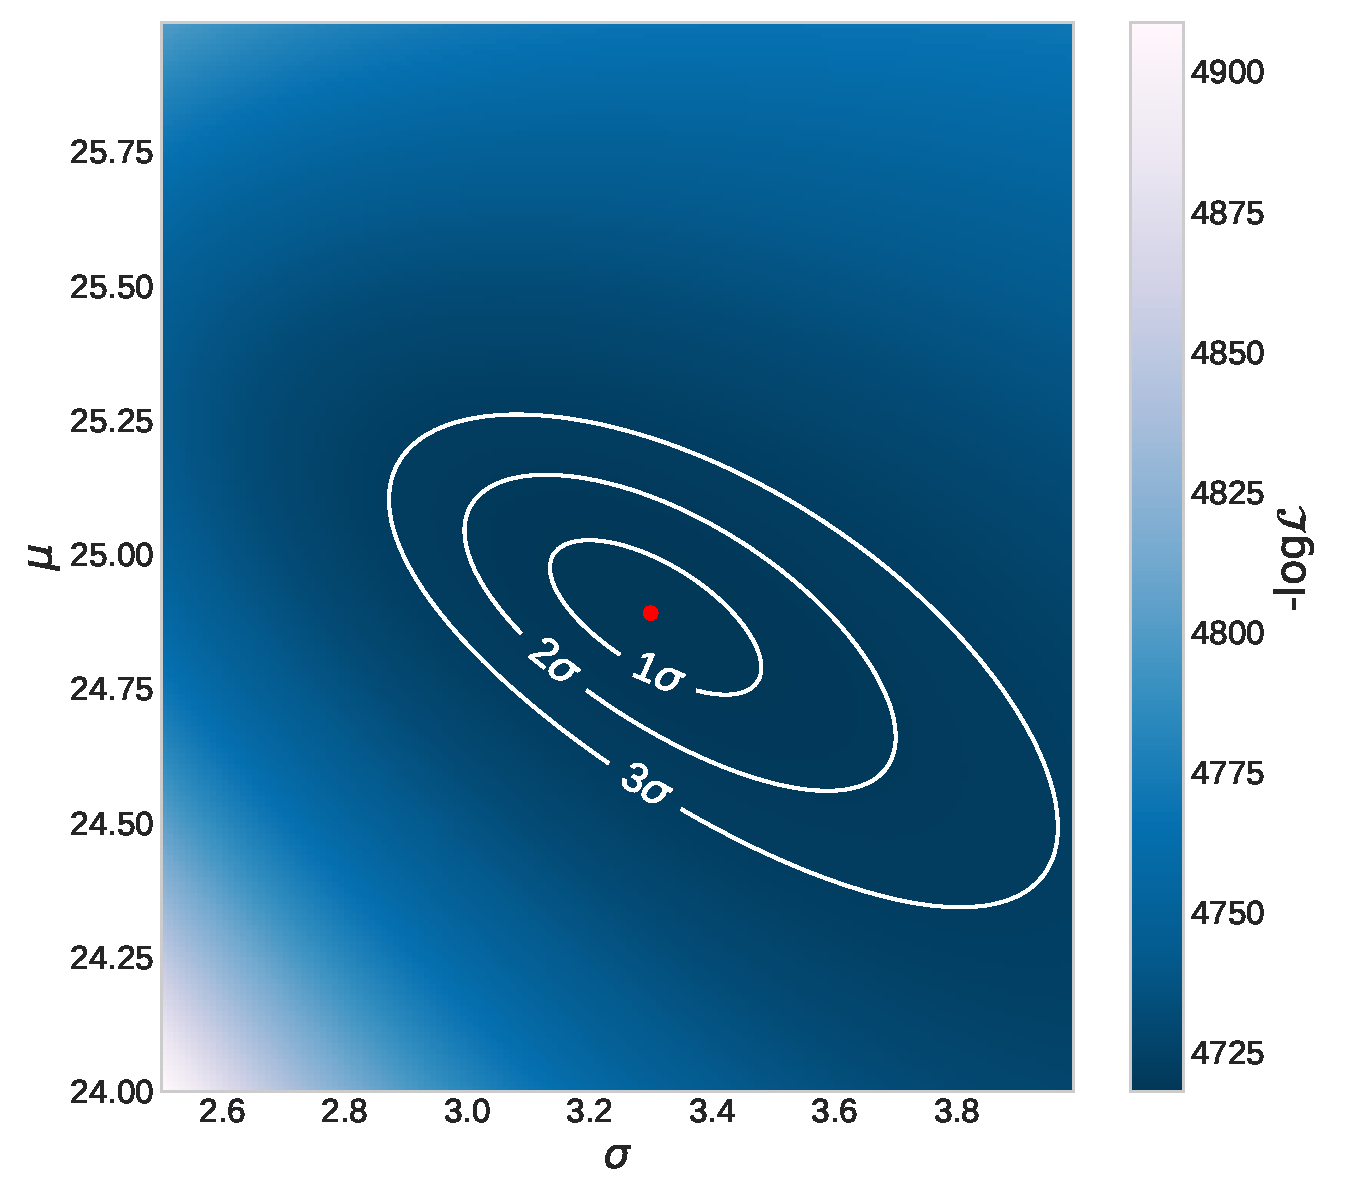
\includegraphics[width=0.45\textwidth]{exampleAnalysis/plots/Likelihood_MC.pdf}
\hfill 
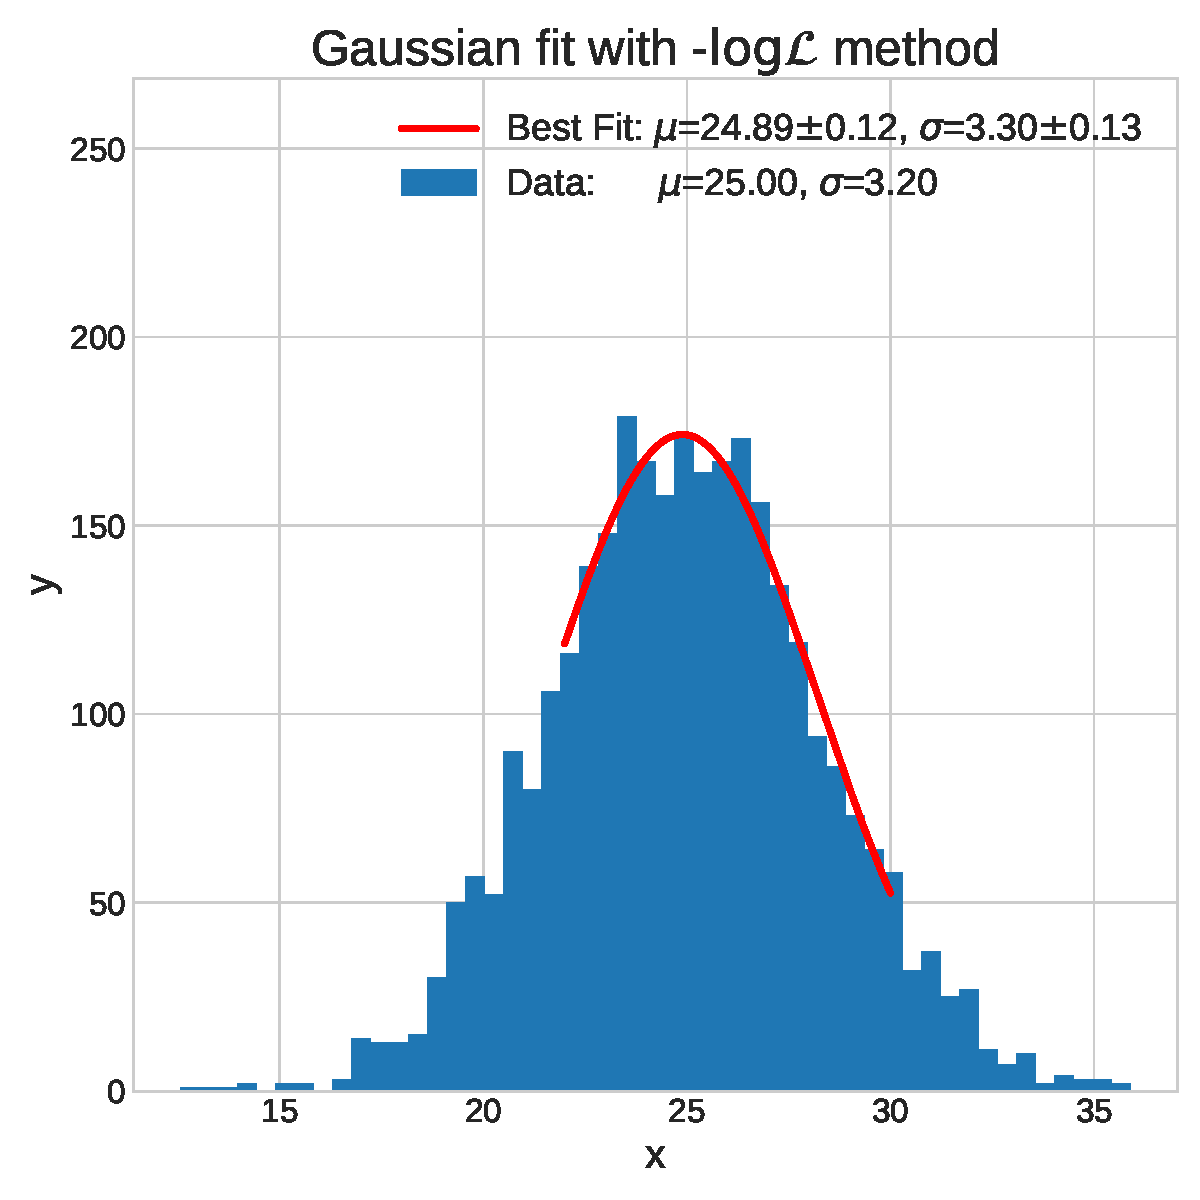
\includegraphics[width=0.45\textwidth]{exampleAnalysis/plots/LLH_Fit_MC.pdf}\\

\textbf{Ajustement des donn{\'e}es:}\\
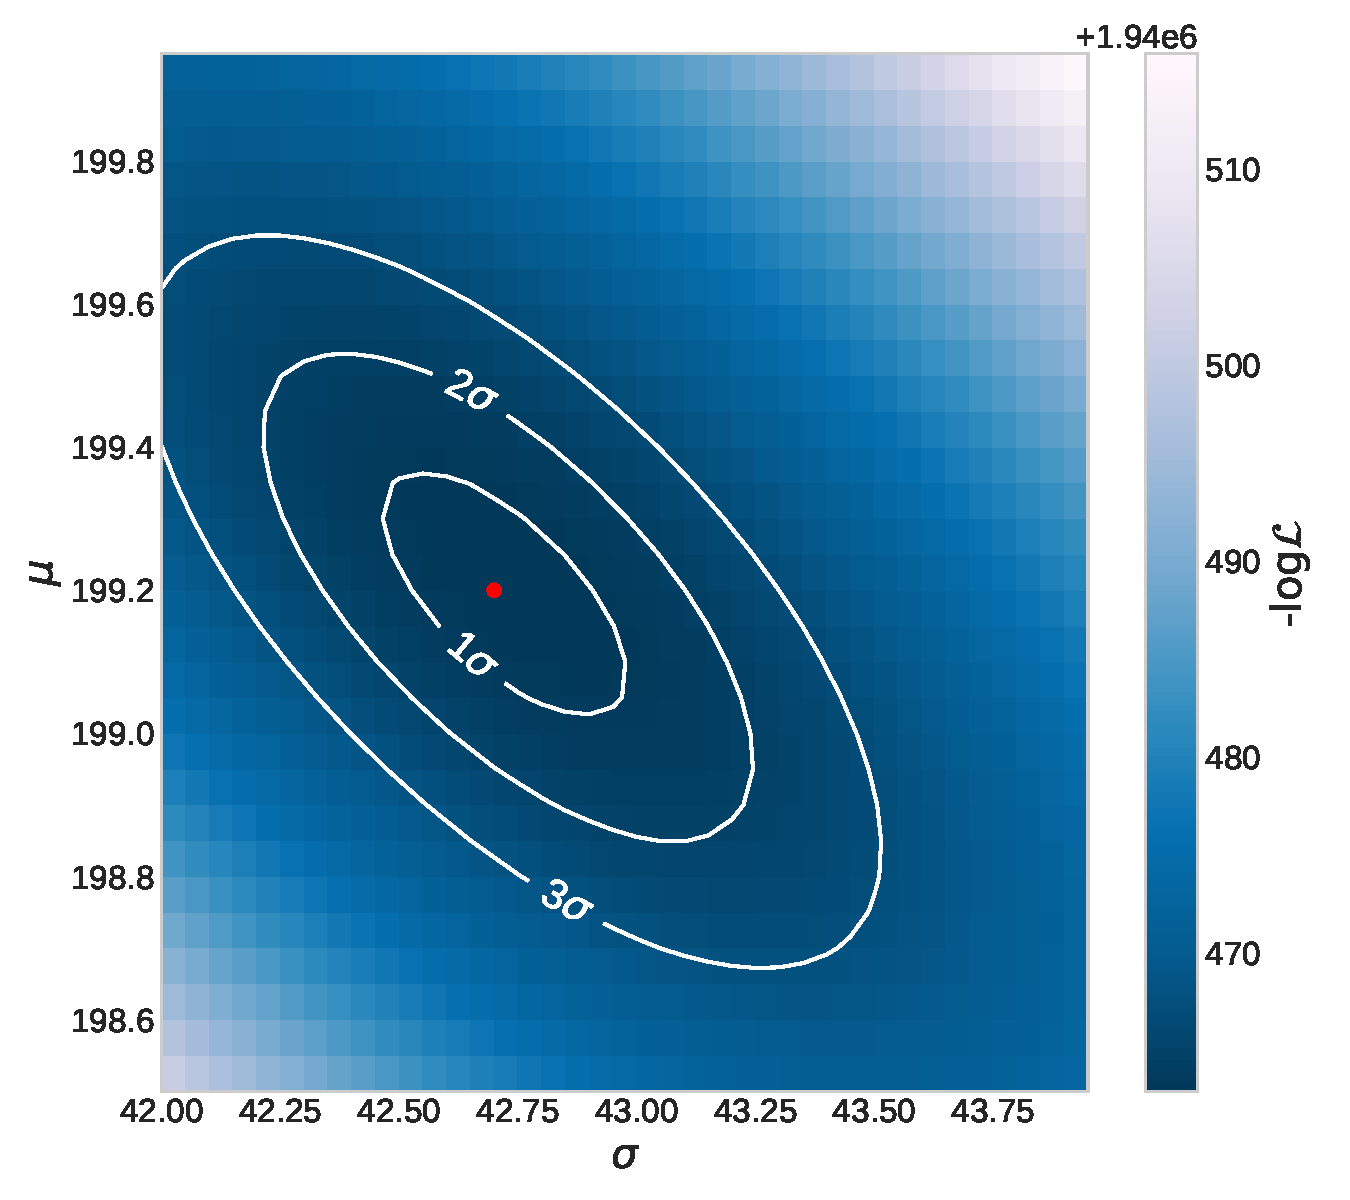
\includegraphics[width=0.45\textwidth]{exampleAnalysis/plots/Likelihood_Data_electron_VME.pdf}\hfill
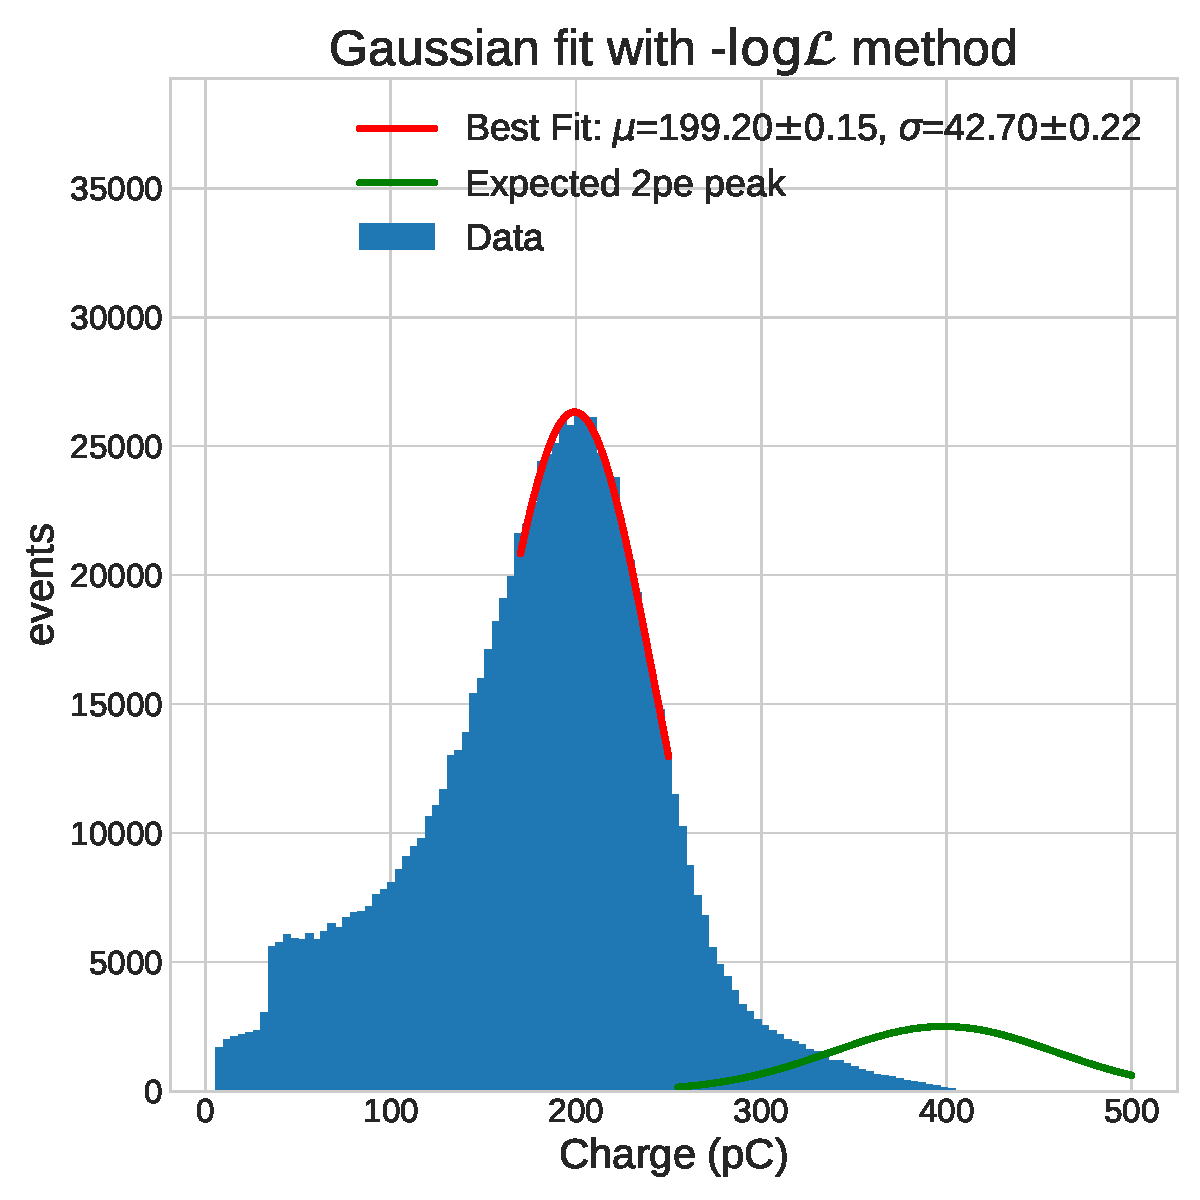
\includegraphics[width=0.45\textwidth]{exampleAnalysis/plots/LLH_Fit_electron_VME.pdf}
\begin{align*}
G &= \mu_{\text{best}}/e = 1242670 \\
\sigma_G &= \sigma_{\text{best}} / \mu_{\text{best}} = 21.44\%
\end{align*}
{\centering
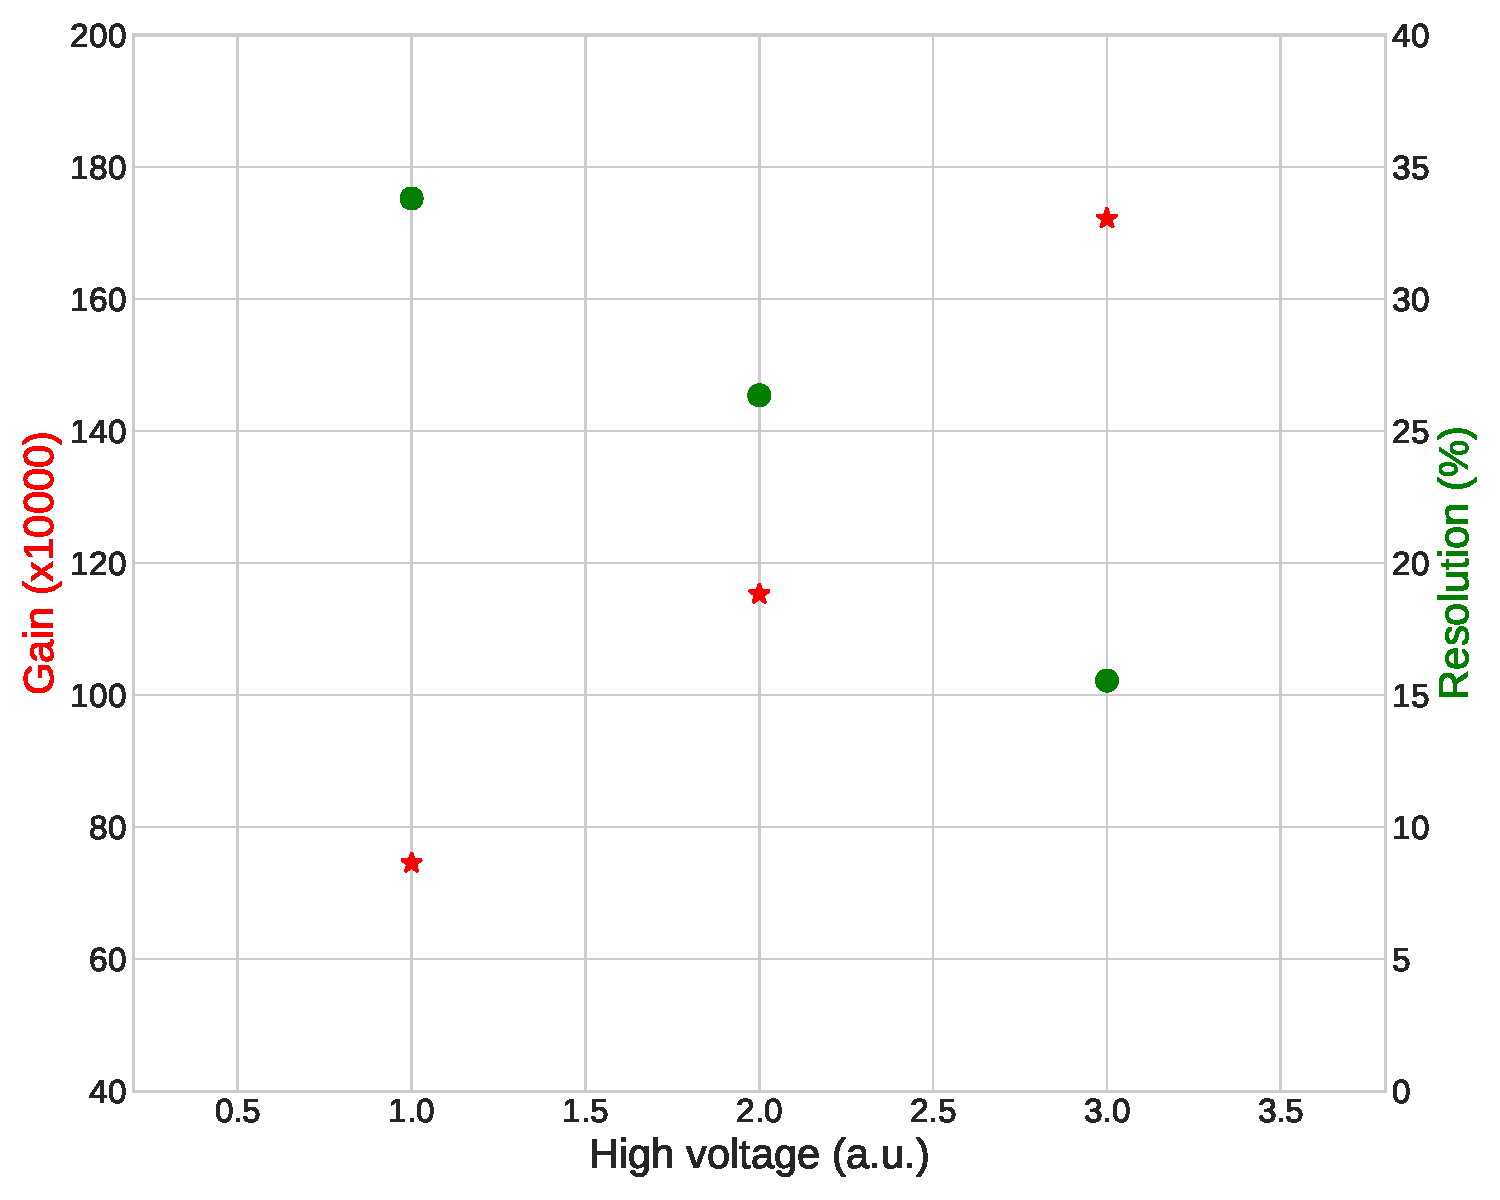
\includegraphics[width=0.7\textwidth]{exampleAnalysis/plots/Electron_Gain_Resolution_HV_VME.pdf}\\}
\end{additional}
}



\section{Dispositif: Effet Tcherenkov par des muons}
\label{sect:Tcherenkov_muon}

L'effet Tcherenkov survient lorsqu'une particule chargée se déplace plus vite que la vitesse de la lumière dans un milieu diélectrique. Ce phénomène résulte de la superposition cohérente d'onde électromagnétique suite à la polarisation du milieu par le passage de la particule chargée. Si la vitesse de la particule est supérieure au ratio $c/n$ (où $n$ est l'indice de réfraction et $c$ la vitesse de la lumière dans le vide), il y a formation d'un cône de lumière avec un angle de demi-ouverture $\Theta_c$ qui suit la relation:

\begin{equation}
    cos\Theta_c = \frac{1}{n\beta}
\end{equation}\\
où $\beta = v/c$, $v$ étant la vitesse de la particule dans le milieu. Le nombre de photons Tcherenkov émis par unité de longueur et de longeur d'onde est donné par la formule de Frank-Tamm:
\begin{equation}
     \frac{d^2N}{dx \, d\lambda} = \frac{2\pi \, \alpha}{\lambda^2} \; (1- \frac{1}{n^2 \, \beta^2} )
\end{equation}\\
avec $\alpha$ étant la constante de structure-fine. Comme le nombre de photons produits est inversement proportionnel à la longueur d'onde, la contribution des petites longueurs d'onde est plus importante.

Compte tenu de leur faible section efficace d'interaction, la détection des neutrinos nécessite un détecteur de grand volume. Cela est réalisé par les détecteurs Tcherenkov en déployant des photo-multiplicateurs (PMs) dans un volume de matériau diélectrique. Chaque PM est contenu dans une bulle de verre sous vide, l'ensemble étant appelé module optique (OM). AMANDA (Antarctic Muon and Neutrino Detector Array) est un télescope à neutrino localisé au Pôle Sud. Lors de sa phase finale, le détecteur était composé de 677 modules optiques (OMs) disposés sur 19 câbles. Ces modules retourne un signal analogique. Après 9 ans d'activité, AMANDA a été officiellement incorporé au détecteur IceCube en 2005. IceCube (figure~\ref{fig:IceCube}) est un détecteur Tcherenkov d'un kilomètre cube enterré dans la glace du Pôle Sud. Il a pour but principal la détection des neutrinos à haute énergie. IceCube est composé de 5160 modules optiques digitaux (DOMs ou Digital Optical Modules) placés sur 86 câbles. Pour constituer un vaste réseaux d'OMs, il nous faut connaître la réponse de chacun de ceux-ci.

\begin{figure}
    \center{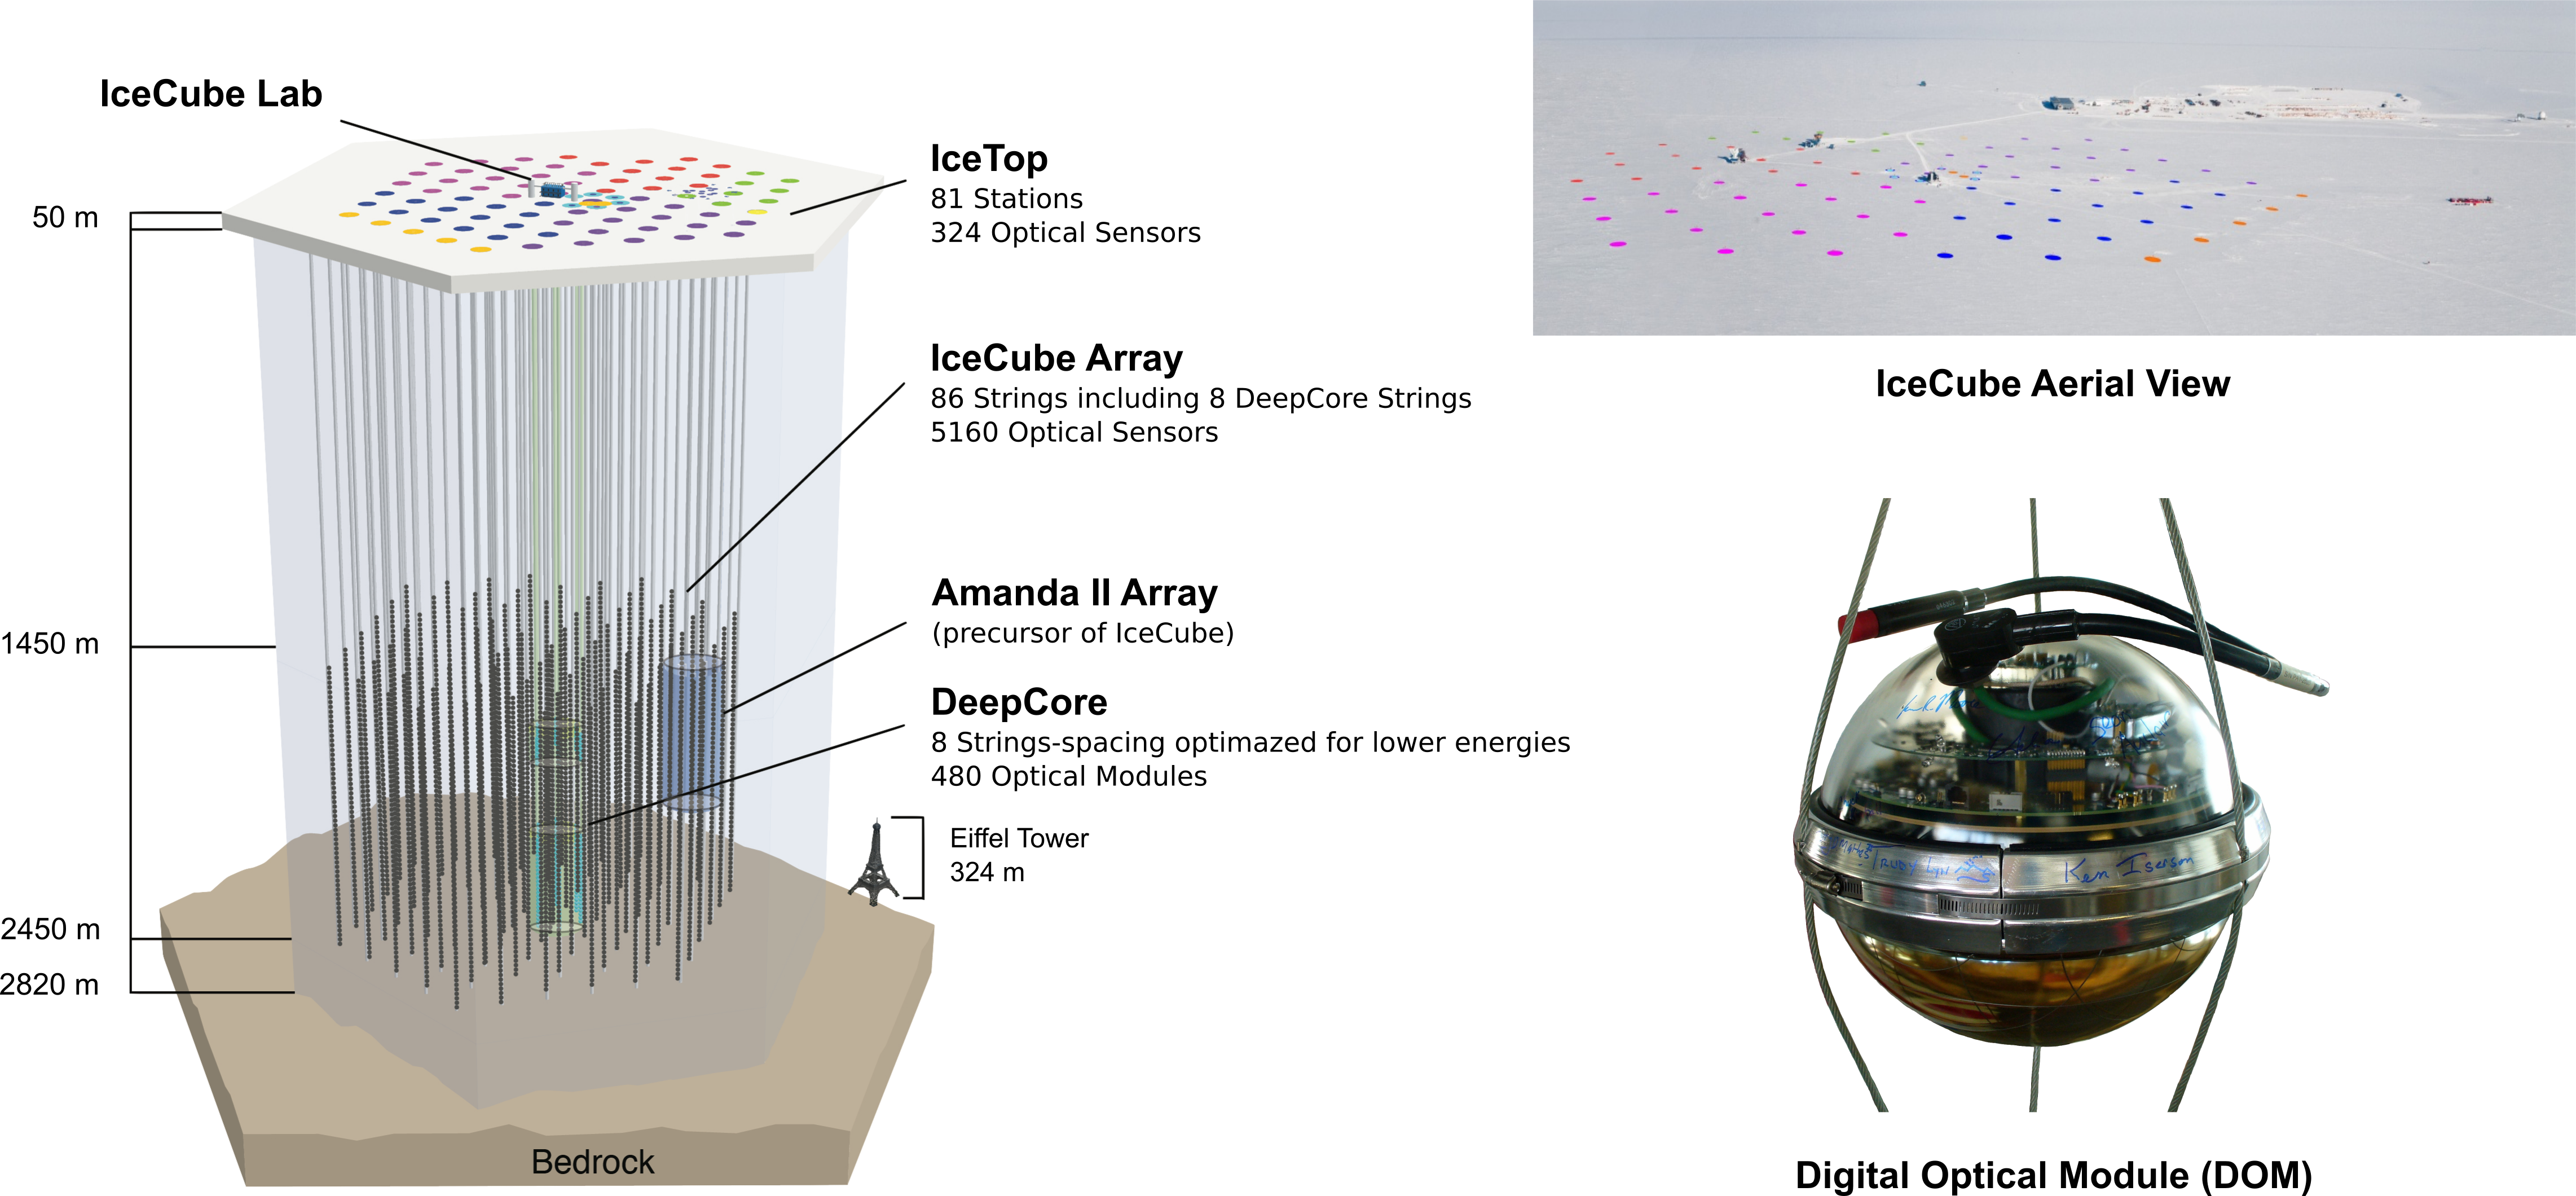
\includegraphics[width=0.8\textwidth]
    {figures/IceCube_Detector.png}}
    \caption{\label{fig:IceCube} Configuration du télescope à neutrinos IceCube.}
\end{figure}

Cette manipulation a pour but la caractérisation d'un module optique (OM) développé pour l'expérience AMANDA. Afin d'étudier les propriétés de cet OM, vous devrez mettre au point le dispositif nécessaire à la prise de mesure. Après avoir pris connaissance avec le dispositif, vous serez ainsi amené à développer vous même la logique d'acquisition des données. Vous analyserez ensuite les données recueillies grâce aux outils statistiques et informatiques que vous aurez vu en cours.

\subsection{Agenda du laboratoire}
\begin{tabular}{p{0.2\linewidth} p{0.8\linewidth}}
Lundi & - Prise de connaissance avec le matériel\newline
		- Vérification du signal analogique des PMs avec l'oscilloscope\newline
		- Implémentation de la table de vérité pour la logique d'acquisition ou trigger\newline
		- Mesure de l'efficacité\\ 

Mardi & - Calibration de l'ADC\newline
		- Préparation de l'acquisition de données\newline
		- Début de l'acquisition de données avec LabView\\ 

Mercredi & - Construction de la logique d'acquisition du bruit de fond\newline
		- Écriture de la table de vérité pour définir un événement du bruit\newline
		- Début de l'acquisition de données pour le bruit de fond\\ 

Jeudi et Vendredi & - Développement d'un programme de génération MC d'une distribution normale\newline
		- Développement des programmes d'analyse\newline
		- Dernier jour pour présenter les résultats des exercices\newline
		- Préparation de la présentation\\
\end{tabular} 

\subsection{Dispositif expérimental}

Pour cette manipulation, nous utilisons les muons atmosphériques afin d'obtenir l'émission Tcherenkov. Ce dispositif est composé de 4 scintillateurs chacun relié à un photo-multiplicateur (PM), d'un OM, une couche de plomb et d'un réservoir d'eau (voir figure \ref{fig:dispo2}). Ce réservoir forme un angle de 45$^{\circ}$ avec la verticale. Les trois premiers PMs (PM1, PM2 et PM3) assurent la direction verticale du muon incident. La présence d'une couche de plomb avant le PM3 nous permet également de vérifier que le muon est suffisamment énergétique pour produire le rayonnement Tcherenkov avec l'angle souhaité. Un 4ème PM est placé au dessus de l'OM et est utilisé comme veto. Puisque les muons sont produits en "paquets", appelés muon bundles, ce veto exclu les évènements de l'OM qui seraient produits par un second muon plutôt que par un photon Tcherenkov.

\begin{figure}
    \centering
	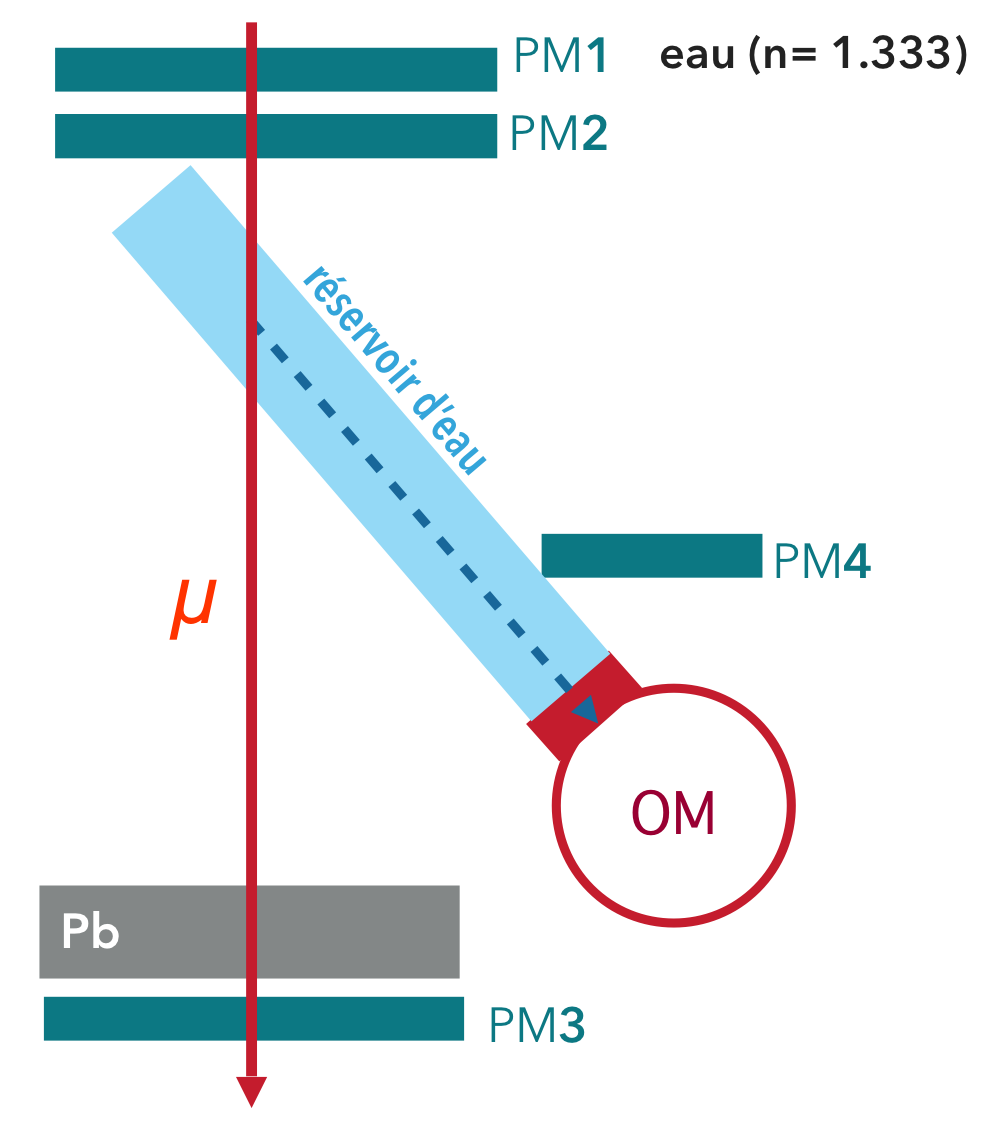
\includegraphics[width=0.5\textwidth]{figures/Dispositif_2.png}
    \caption{Dispositif expérimental de l'effet Tcherenkov produit par des muons.}
    \label{fig:dispo2} 
\end{figure}

\subsection{Exercices Pr\'eparatoires}

\subsubsection{Exercice 1}
Calculez quelle sera l'angle d'\'emission du rayonnement Tcherenkov \'emis dans l’eau par des muons ($m_\mathrm{\mu} = 0.106$\,GeV/$c^2$) de $1.5$\,GeV/$c$ de quantité de mouvement, sachant que l'indice de r\'efraction de l'eau \`a $20^\circ$C est $1.333$.

\ifthenelse{\boolean{showAdditional}}{
\begin{additional}
\begin{align*}
\begin{split}
\beta &= \frac{v}{c} = \frac{pc}{E}\\
 &= \frac{pc}{\sqrt{p^2c^2+m_\mathrm{\mu}^2c^4}}\\
 &= 0.9975\\
\end{split}
\quad
\begin{split}
\cos\Theta_\mathrm{c} &= \frac{1}{\beta n}\\
 \Theta_\mathrm{c} &= \arccos\frac{1}{0.9975\cdot1.33}\\
 &= \boxed{41.2^\circ} 
\end{split}
\end{align*}
\end{additional}
}

\subsubsection{Exercice 2}
Calculer l'ordre de grandeur du nombre de photons \'emis entre $350$ et $500$\,nm par un muon de $1.5$\,GeV/$c$ de quantité de mouvement traversant un réservoir d'eau de 10\,cm d'\'epaisseur. Pour ce domaine de longueurs d’onde, l'indice de r\'efraction d'eau varie de moins de 1\% et peut \^etre consid\'er\'e constant ($1.333$). N\'egliger la perte d'\'energie du muon dans l'eau.\\ $\alpha = 1/137$

\ifthenelse{\boolean{showAdditional}}{
\begin{additional}
Formule de \emph{Frank-Tamm}:
\begin{align*}
\frac{\mathrm{d}N}{\mathrm{d}x} &= \int_{\lambda_0}^{\lambda_1} \frac{2\pi\alpha z^2}{\lambda^2} \sin^2\Theta_\mathrm{c} \mathrm{d}\lambda\\
&=\frac{0.868\pi}{137}\int_{350\,\mathrm{nm}}^{500\,\mathrm{nm}}\frac{\mathrm{d}\lambda}{\lambda^2}\\
N&=\frac{0.868\pi}{137}\cdot\left(\frac{1}{350\,\mathrm{nm}}-\frac{1}{500\,\mathrm{nm}}\right)\cdot1\,\mathrm{cm}\\
&=\boxed{1706}
\end{align*}
\end{additional}
}

\subsubsection{Exercice 3}
Les photons Tcherenkov sont produits \`a 1\,m de l'OM, devant lequel se trouve un collimateur de 10\,cm de diam\`etre. Combien de photoélectrons l'OM peut-il enregistrer par muon, en supposant la transmittance $T$ \`a 90\%, l'efficacit\'e quantique est de $\epsilon_\mathrm{q}=15\%$? L'absorption de photons dans l'eau peut \^etre négligée, ainsi que la réflexion de photons au bord du réservoir.

\ifthenelse{\boolean{showAdditional}}{
\begin{additional}
Avec $N_\mathrm{\gamma}^{\mathrm{eau}}$ trouv\'e avant, on obtient:
\begin{align*}
N_{\mathrm{pe}} &= \epsilon_\mathrm{q} \cdot T \cdot N_\mathrm{\gamma}^{\mathrm{OM}}\\
 &= \epsilon_\mathrm{q} \cdot T \cdot \frac{10\,\mathrm{cm}}{2\pi \cdot 100\,\mathrm{cm} \cdot\sin\Theta_\mathrm{c}} \cdot N_\mathrm{\gamma}^{\mathrm{eau}}\\
&= \boxed{5.56}
\end{align*}
\end{additional}
}

\subsection{Prise de mesure}

Pour cette manipulation, il vous est demandé de préparer le dispositif expérimental nécessaire à la prise de mesure. Cela implique, dans un premier temps, de :\\

\begin{center}
\fbox{
\begin{minipage}{0.75\textwidth}
\textbf{Se familiariser avec le dispositif :} 
\begin{quote}
\begin{itemize}
\item vérifier le signal des différents PMs et de l'OM
\item étudier l'efficacité des PMs
\item calibrer l'ADC
\item développer la logique d'acquisition de données
\item mesurer le bruit de fond
\end{itemize}
\end{quote}
\end{minipage}
}
\end{center}

\subsubsection{Vérification du dispositif}
Dans un premier temps, allumez votre dispositif et allumez la haute tension aux bornes des PMs. Veillez ne pas changer la tension indiquée afin de ne pas endommager les PMs.\\
A l'aide de l'oscilloscope, vérifiez le signal provenant des différents photo-multiplicateurs (PMs) et de l'OM. Transformez ensuite votre signal analogue en signal digital à l'aide du discriminateur et observez celui-ci sur l'oscilloscope.

\subsubsection{Mesure de l'efficacité}

Il vous est ensuite demandé de mesurer l'efficacité d'un des PMs présents dans votre dispositif. Vous devrez faire cette mesure en faisant varier dans un premier temps le seuil du PM pour lequel vous mesurer l'efficacité. Une fois la valeur optimale du seuil trouvée, répétez le processus en faisant cette fois varier la tension appliquée sur le PM en question. Pour ces deux mesures, veillez également à mesurer le taux d'évènements détectés par le PM dont vous mesurez l'efficacité. Pour effectuer ces mesures, vous avez à votre disposition un scaler NIM. De quel PM allez-vous mesurer l'efficacité ?

\ifthenelse{\boolean{showAdditional}}{
\begin{additional}
\begin{itemize}
\item Mesure de l'efficacité de PM2
\item Logique : (PM1 \& PM2 \& PM3) et (PM1 \& PM3)
\item Mesure du rate de PM2
\end{itemize}
\end{additional}
}

\subsubsection{Calibration de l'ADC}

Nous allons à présent procéder à la calibration du convertisseur analogique-numérique (ADC ou Analogue-to-Digital Converter). En effet, l'ADC vous donne des valeurs en ADC channel, il vous faut donc connaître à quelle charge équivaut un ADC channel.

Pour cette calibration, il faut fournir une charge connue et constante à l'ADC. Pour cela, vous avez à votre disposition un générateur de courant continu. Comment allez-vous procéder ? 

\ifthenelse{\boolean{showAdditional}}{
\begin{additional}
\begin{itemize}
    \item Charge de l'ADC de l'ordre du pC $\to$ $Q\sim100$\,pC 
    \item Utilisation d'une résistance: $U = RI$ avec $R = 2.2$\,k$\mathrm{\Omega}$
    \item Sachant que $Q = I\mathrm{\Delta}t$, déterminer $\mathrm{\Delta}t$
    \item Le gate est ensuite créé à l'aide du dual-timer
\end{itemize}
\end{additional}
}

\subsubsection{Prise de données}

Afin de prendre les données nécessaires à la caractérisation de l'OM, nous devons réfléchir à la logique d'acquisition. Nous allons utiliser l'ADC que nous venons de calibrer et lui fournir le signal de l'OM ainsi qu'une porte logique (gate). Pour créer ce gate, nous avons besoin des modules logiques. Il nous faut réfléchir aux conditions dans lesquelles ont veut déclencher la prise de mesure. En d'autres termes, quand-est-ce que le signal de l'OM nous intéresse? Une fois que cela est clair, vous pouvez l'implémenter à l'aide des modules logiques. Il vous faudra ensuite vérifier que le signal de l'OM et votre porte logique sont en coïncidence à l'aide de l'oscilloscope. Lorsque vous avez effectué cette vérification, reliez le gate et le signal de l'OM à l'ADC pour commencer la prise de mesure.

\textbf{Attention :} Pour la manipulation utilisant les muons, veillez à changer le nom du fichier pour ne pas qu'il soit écrasé lors de la prise de mesure suivante.

\ifthenelse{\boolean{showAdditional}}{
\begin{additional}
\begin{itemize}
\item \textbf{Gate :} (PM1 \& PM2 \& PM3) \& (OM \& !PM4)
\item Faire passer le gate dans le dual-timer pour avoir des fenêtres de taille constante
\item Vérifier que l'OM est en même temps que le gate
\item On veut aussi le muon rate ($\sim 1$\,Hz) donc on passe (PM1 \& PM2 \& PM3) dans le scaler relié au PC
\item Donner le gate et le signal à l'ADC (taux de coïncidence $\sim 0.2$\,Hz) et commencez la prise de mesure
\end{itemize}
\end{additional}
}

\subsubsection{Mesure du bruit de fond}

Intéressons nous au bruit de fond présent dans votre manipulation. Nous voulons connaître le taux de fausses coïncidences, càd les cas où l'OM nous envoie un signal qui n'est pas dû à un photon Tcherenkov alors que notre porte logique s'est déclenchée.

Dans un premier temps, il vous faut réfléchir à la manière dont vous pouvez implémenter la prise de mesure du bruit de fond. Une fois cette méthode mise en place, vous pouvez démarrer l'acquisition du bruit de fond. A l'aide de l'oscilloscope, pensez toutefois à vérifier que le signal de l'OM et votre gate arrivent en même temps à l'ADC.

\ifthenelse{\boolean{showAdditional}}{
\begin{additional}
\begin{itemize} 
\item \textbf{Gate :} (PM1 \& PM2 \& PM3) \& (OM$_{\mathrm{delayed}}$) \& !(PM4)
\begin{quote}
    A l'aide d'un câble, on ajoute un délai de 50\,ns sur l'OM avant la logique\\
    Cela permet la mesure du taux de fausses coïncidences\\
    On obtient un taux très faible avec $\sim 1$ évènement par heure
\end{quote}

\item \textbf{Gate :} !(PM1 \& PM2 \& PM3) \& (OM) \& !(PM4)
\begin{quote}
    On s'intéresse ici à tous les évènements de l'OM qui ne sont pas dû à un photon Tcherenkov\\
    A partir de cela, on peut néanmoins calculer le taux de fausses coïncidences\\
    $R_{\mathrm{fc}} = 2 \cdot R_{\mathrm{mu}} \cdot R_{\mathrm{bf}} \cdot f $ \\
    où $R_{\mathrm{fc}}$ est le taux de fausse coïncidence, $R_{\mathrm{\mu}}$ le taux de muons et $f$ est la fenêtre de temps.
\end{quote}
\end{itemize}
\end{additional}
}

\subsection{Analyse de donn\'ees}

A présent, nous pouvons nous concentrer sur l'analyse des données dans le but de caractériser l'OM.

En vous basant sur les données, vous devrez calculer:\\
\begin{center}
\fbox{
\begin{minipage}{0.75\textwidth}
\textbf{Dispositif muon :}
\begin{itemize}
\item le gain $G$ de l'OM,
\item la r\'esolution $\sigma_\mathrm{G}$ de l'OM,
\item le nombre moyen de photo-\'electrons $\langle n_{\mathrm{pe}}\rangle$ produit par trigger dans l'OM.
\end{itemize}
\end{minipage}
}
\end{center}

\ifthenelse{\boolean{showAdditional}}{
\begin{additional}
\textbf{Validation de la procedure d'adjustement:}\\
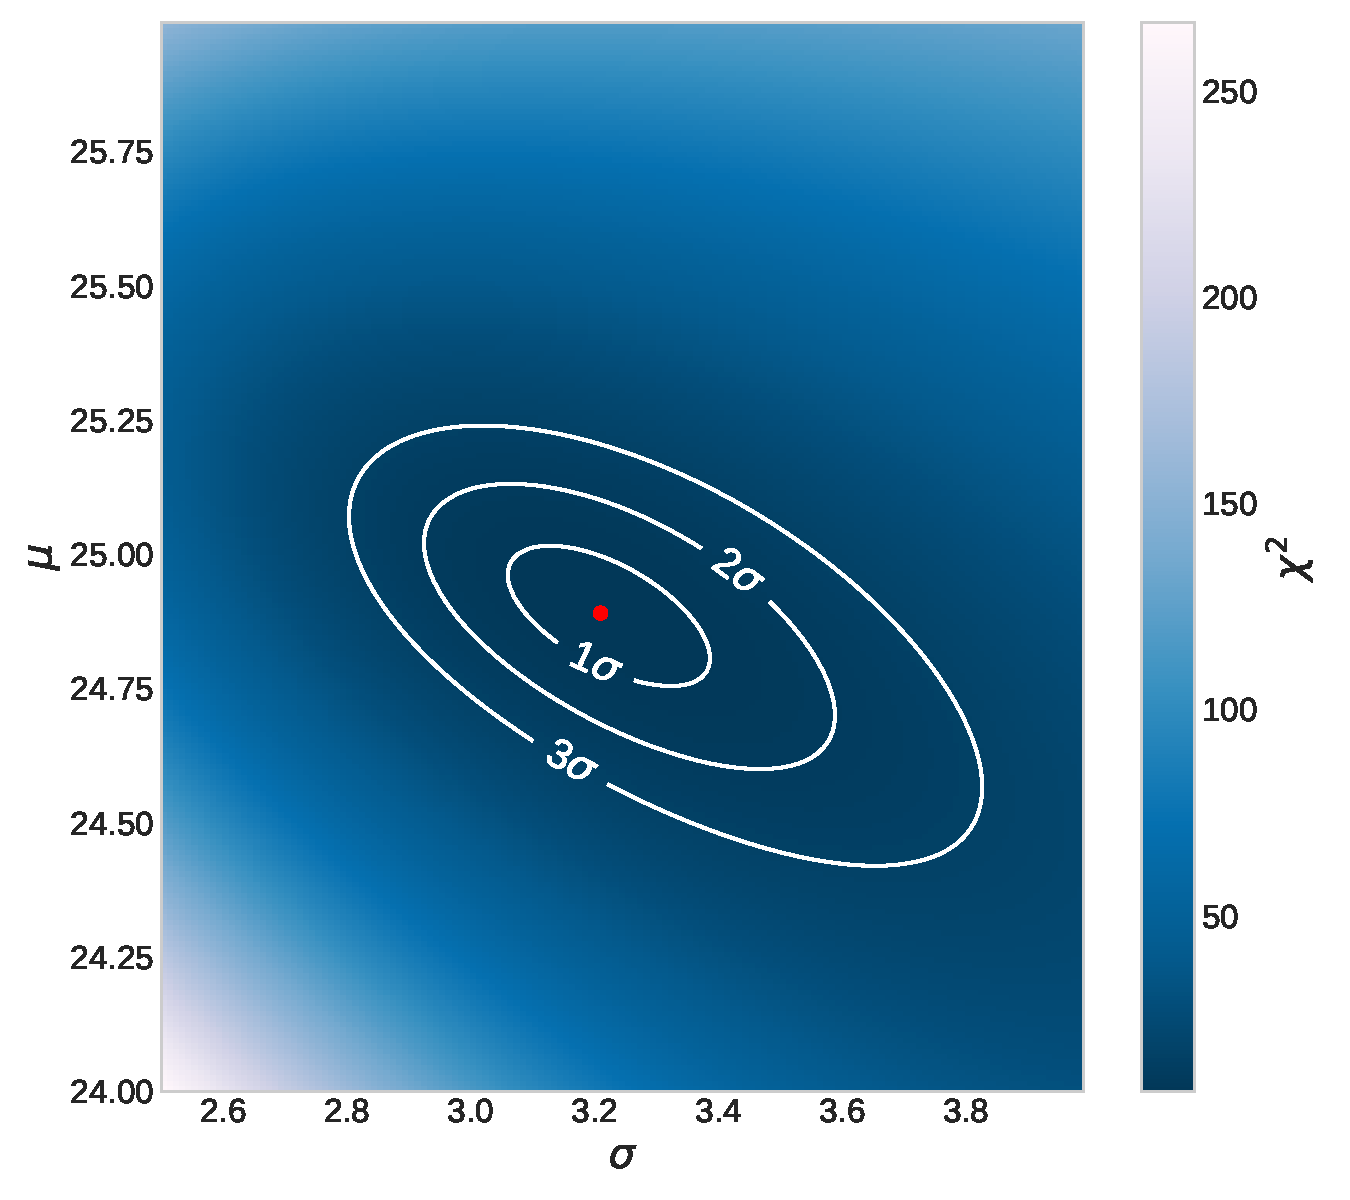
\includegraphics[width=0.45\textwidth]{exampleAnalysis/plots/Chi2_MC.pdf}
\hfill 
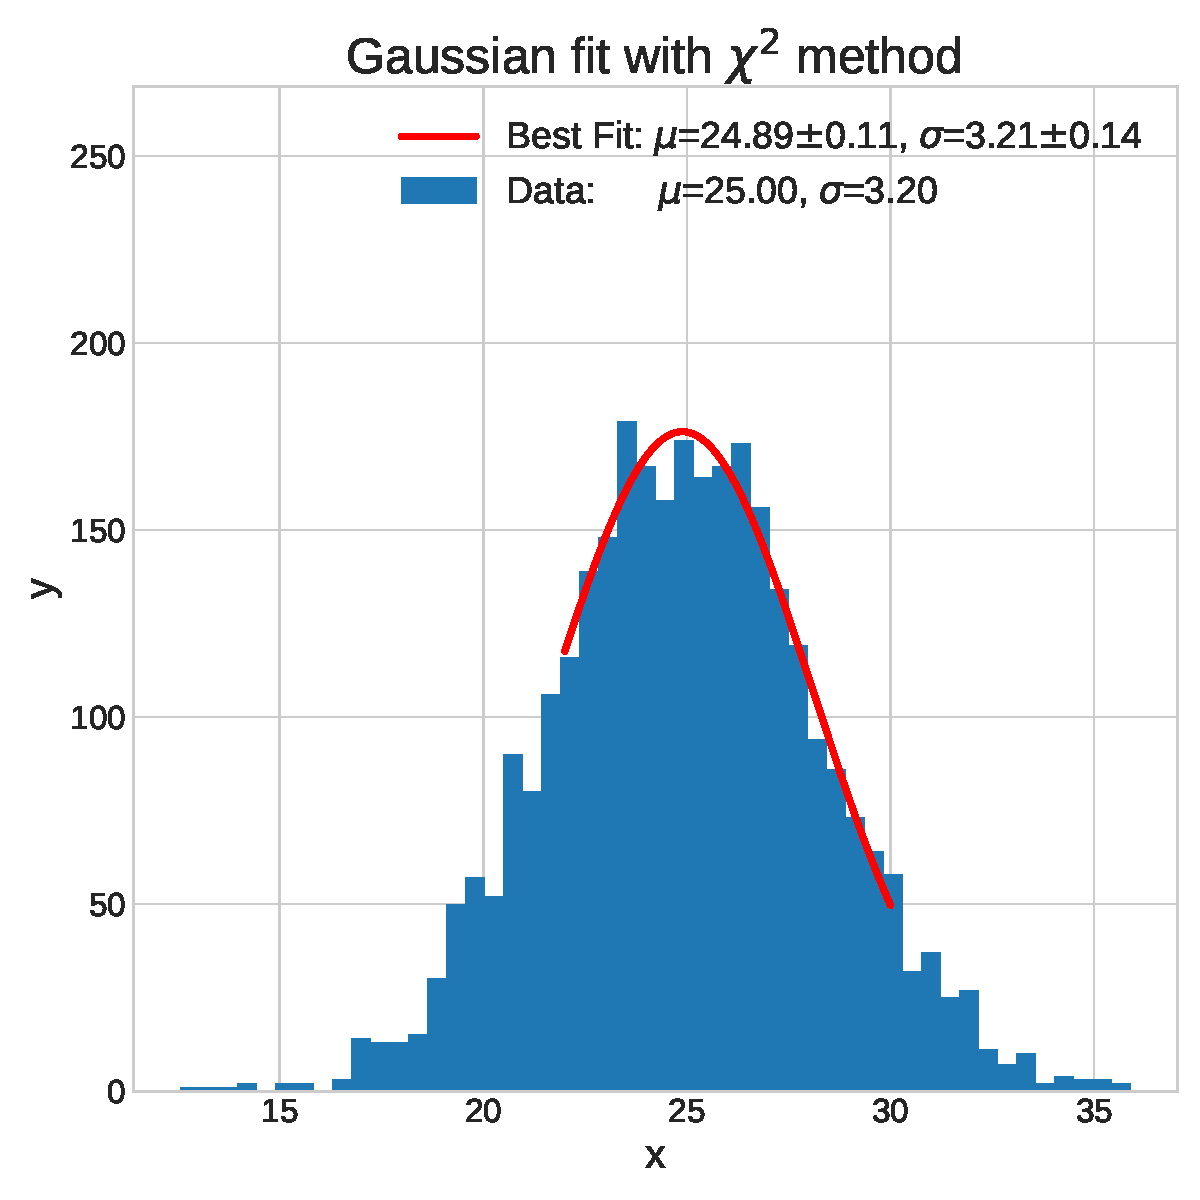
\includegraphics[width=0.45\textwidth]{exampleAnalysis/plots/Chi2_fit_MC.pdf}\\

\textbf{Ajustement des donn{\'e}es:}\\
\begin{align*}
G &= \mu_{\text{best}}/e = ... \\
\sigma_G &= \sigma_{\text{best}} / \mu_{\text{best}} = ...\%\\
\langle n_{\mathrm{pe}}\rangle &= ...
\end{align*}
\end{additional}
}



\section{Dispositif: Temps de vie du muon}
Cette manipulation a pour but la mesure du temps de vie du muon, en utilisant
les muons produits dans les rayons cosmiques. L'exp\'erience ne mesure pas la
charge des particules; on ne peut donc pas diff\'erencier les muons et
leur anti-particule avec le dispositif propos\'e.

Le dispositif (voir figure~\ref{fig:TpsVieMuon_disp}) est compos\'e de 4 grands ($\sim$ 1m$^2$) scintillateurs (voir section
2.1) coupl\'es \`a un (parfois deux) photomultiplicateurs (voir section 2.2).

\begin{figure}[!h]
    \centering
	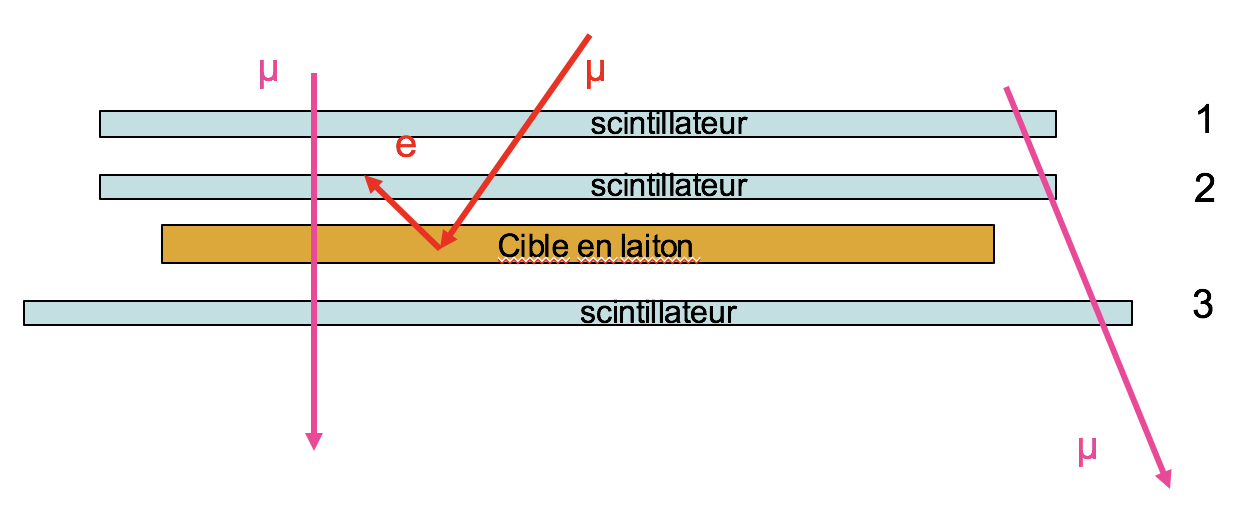
\includegraphics[width=\textwidth]{figures/Schema-Tps-de-vie.png}
    \caption{Schema du dispositif pour la mesure du temps de vie du muon.}
    \label{fig:TpsVieMuon_disp} 
\end{figure}

Le temps de vie \'etant mesur\'e pour des muons au repos, les scintillateurs sont plac\'es de part et d'autre d'une cible en laiton.
Une fois au repos, le muon se d\'esint\'egrera (avec une probabilit\'e de 98$\%$) en un
\'electron avec l'\'emission de deux neutrinos, selon la r\'eaction
$\mu^+ \rightarrow e^+ \nu_e \bar{\nu_{\mu}}$, avec un temps de vie moyen de 2.2 $\mu$s.
Vous allez donc mesurer pour chaque muon qui s'arr\^ete dans la cible le temps
entre la d\'etection de l'arr\^et du muon dans la cible et la d\'etection de
l'\'emission de l'\'electron (notre dispositif est incapable de d\'etecter
les neutrinos).

Le temps de d\'esint\'egration sera mesur\'e \`a l'aide d'un TDC (voir section).
Le TDC ne fonctionne qu'avec des signaux digitaux répondant au standard NIM;
il vous faudra donc cr\'eer de tels signaux \`a  partir des signaux analogiques
qui sortent des photomultiplicateurs. Les signaux des photomultiplicateurs seront convertis en signaux NIM grâce à des discriminateurs. Avec ces signaux vous
pourrez concevoir une logique dite de declenchement (trigger) pour enregistrer
le temps de d\'esint\'egration sur le PC d'acquisition et pour ne pas
enregistrer n'importe quel temps entre deux signaux consécutifs qui pourraient
\^etre dus \`a du bruit \'electronique ou \`a des particules ne s'arr\^etant pas dans la cible.

Avant de concevoir cette logique de déclenchement de l'acquisition et de l'enregistrement des donn\'ees vous devrez effectuer une s\'erie de v\'erifications
et de calibrations pour vous assurer que les donn\'ees qui seront enregistrées
ont du sens:

\begin{center}
\fbox{
\begin{minipage}{0.75\textwidth}
\textbf{Les grandes étapes de la partie instrumentale :} 
\begin{quote}
  \begin{itemize}
    \item V\'erifier les signaux de tous vos PMs
\item étudier l'efficacité des PMs et mesurer le bruit de fond
\item calibrer le TDC
\item développer la logique d'acquisition de données
\item tester la logique avant de lancer l'acquisition pour la nuit
\end{itemize}
\end{quote}
\end{minipage}
}
\end{center}

\subsection{Vérification du dispositif}
\textbf{Avec l'aide d'un assistant} régler les tensions des PMs de manière à 
avoir des signaux observables \`a l'oscilloscope. Les tensions de fonctionnement des PM du dispositif dit ``vieux'' et qui possède 8 PMs sont de l'ordre de 2000 à 2200V. \textbf{Ne dépassez en aucun cas 2200V sur ce dispositif}.

Une fois que vous avez identifi\'e les signaux des PMs à l'oscilloscope, observez-les et prenez note de leurs caract\'eristiques (amplitude, temps de 
mont\'ee, dur\'ee, etc.).

Vérifier qu'ils sont en temps. En effet pour pouvoir identifier un muon ou un \'electron
avec votre dispositif vous utiliserez le fait que les signaux de
2 PMs attach\'es au m\^eme scintillateur sont en coincidence temporelle.

\subsection{Mesure de l'efficacité et du taux d'événements}

Il vous est ensuite demandé de mesurer l'efficacité d'au moins un des PMs 
présents dans votre dispositif, en particulier un PM situ\'e au-dessus de la 
cible. Vous effectuerez la mesure de l'efficacité en fonction de deux paramètres: (1) la tension de fonctionnement du PM en question et (2) le seuil de 
déclenchement du discriminateur attaché à ce PM.
\textbf{Attention, on ne fait varier qu'un paramètre à la fois !}

Simultanément, on vous demande de mesurer le taux d'événements détectés par le 
PM que vous testez. Notez qu'au maximum ce taux peut atteindre 1 kHz.

Pour ces mesures, appliquez une tension de l'ordre de 2100 V sur les autres PMs et un seuil de l'ordre de 50 mV.

Finalement, pour rappel, toute mesure expérimentale doit être accompagnée de son erreur de mesure !

\subsection{Calibration du TDC}
Comme vous utiliserez un TDC (voir section 2.3) pour mesurer les temps de désintégration des muons,il est important de vérifier que celui-ci est toujours bien calibré. Pour cela vous 
allez envoyer de manière périodique un signal 'start' pour enclencher le TDC, suivi d'un signal 'stop' pour arrêter le TDC. Vous utiliserez pour ce faire un module NIM appelé TIMER, en boucle, avec lequel vous pouvez régler les délais entre
le signal \textit{start} et le signal \textit{stop} ainsi que la période de répétition de cette séquence.
Pour calibrer votre TDC, choisissez des temps qui sont du même ordre de grandeur 
que les temps que vous vous apprêtez à mesurer avec votre dispositif.

\subsection{Prise de données}
Avant de commencer à câbler votre logique pour la prise de données, dessiner votre logique sous forme d'un ``bloc diagram'' sur une feuille de papier, pour
bien visualiser le chemin suivi par chaque signal. Faites vérifier votre logique
par un assistant avant de câbler !
Typiquement, les seuils des discriminateurs des PM au-dessus de la cible sont relevés (en valeur absolue) pour réduire le bruit de fond, alors que ceux des  
discriminateurs des PM en-dessous de la cible sont les plus bas possible. Ces 
signaux sont aussi parfois élargis en temps par rapport à ceux des PMs du dessus; \textbf{pourquoi ?}
\newline
 \textbf{Important:} avant de lancer l'acquisition des données pour toute une nuit, faites toujours un essais de plusieurs dizaines de minutes, pour vous assurez que
votre dispositif fonctionne bien. Vous devez vous attendre à un taux de une à 
deux désintégrations de muons par minute !

\subsection{Analyse des données}
Pour l'analyse des données vous programmerez votre propre code d'ajustement, 
par la méthode des moindres carrés ou le maximum de vraisemblance, au choix.
Avant de vous lancez dans l'écriture du code, faites réviser vos formules mathématiques et prenez garde à la normalisation des probabilités et/ou des histogrammes.
Pour exercer votre code d'analyse et le debogguer, vous devrez écrire un autre
programme pour simuler les temps de vie des muons, soit par la méthode inverse, soit par la méthode dite ``hit and miss'', au choix. Les temps de vie doivent être écrits dans un fichier excatement comme le sont les temps de vie de votre
expérience; ainsi votre code d'analyse pourra traiter de la même  manière vos données simulées et vos données réelles.



\section{Dispositif: L'arche cosmique}
\label{sect:Muon_arche}

Cette expérience a pour objectif la mesure de la distribution angulaire des muons atmosphériques.
Au cours de ce laboratoire, vous apprendrez à utiliser et caractériser des scintillateur et photomultiplicateurs dans le cadre de la détections de muons.
Vous calibrerez le dispositif et développerez la logique d'acquisition des données.
Finalement, vous analyserez celles-ci grâce aux outils statiques vus au cours théorique.

\subsection{Agenda du laboratoire}
\begin{tabular}{p{0.2\linewidth} p{0.8\linewidth}}
Lundi & - Familiarisation avec le matériel\newline
		- Vérification des signaux analogiques des PMs à l'oscilloscope\newline
		- Mise en temps des signaux\newline
		- Mesure de l'efficacité des PMs en fonction de la tension et du seuil\\

Mardi & - Mesure de l'efficacité des PMs en fonction de l'angle zénithal\newline
		- Introduction au TDC et \textit{dual-timer}\newline
		- Éventuellement, première calibration de la position en fonction de la différence de temps d'arrivée des signaux\\

Mercredi & - Calibration de la position en fonction de la différence de temps d'arrivée des signaux\newline
		- Mesure de la vitesse de la lumière dans les guides de lumières\newline
		- Début de l'acquisition de données\\

Jeudi et Vendredi & - Mise en forme, préparation des données\newline
		- Développement d'une simulation Monte-Carlo\newline
		- Développement du programme d'analyse\newline
		- Préparation de la présentation\\
\end{tabular} 

\subsection{Dispositif expérimental}

\begin{figure}
\begin{center}
    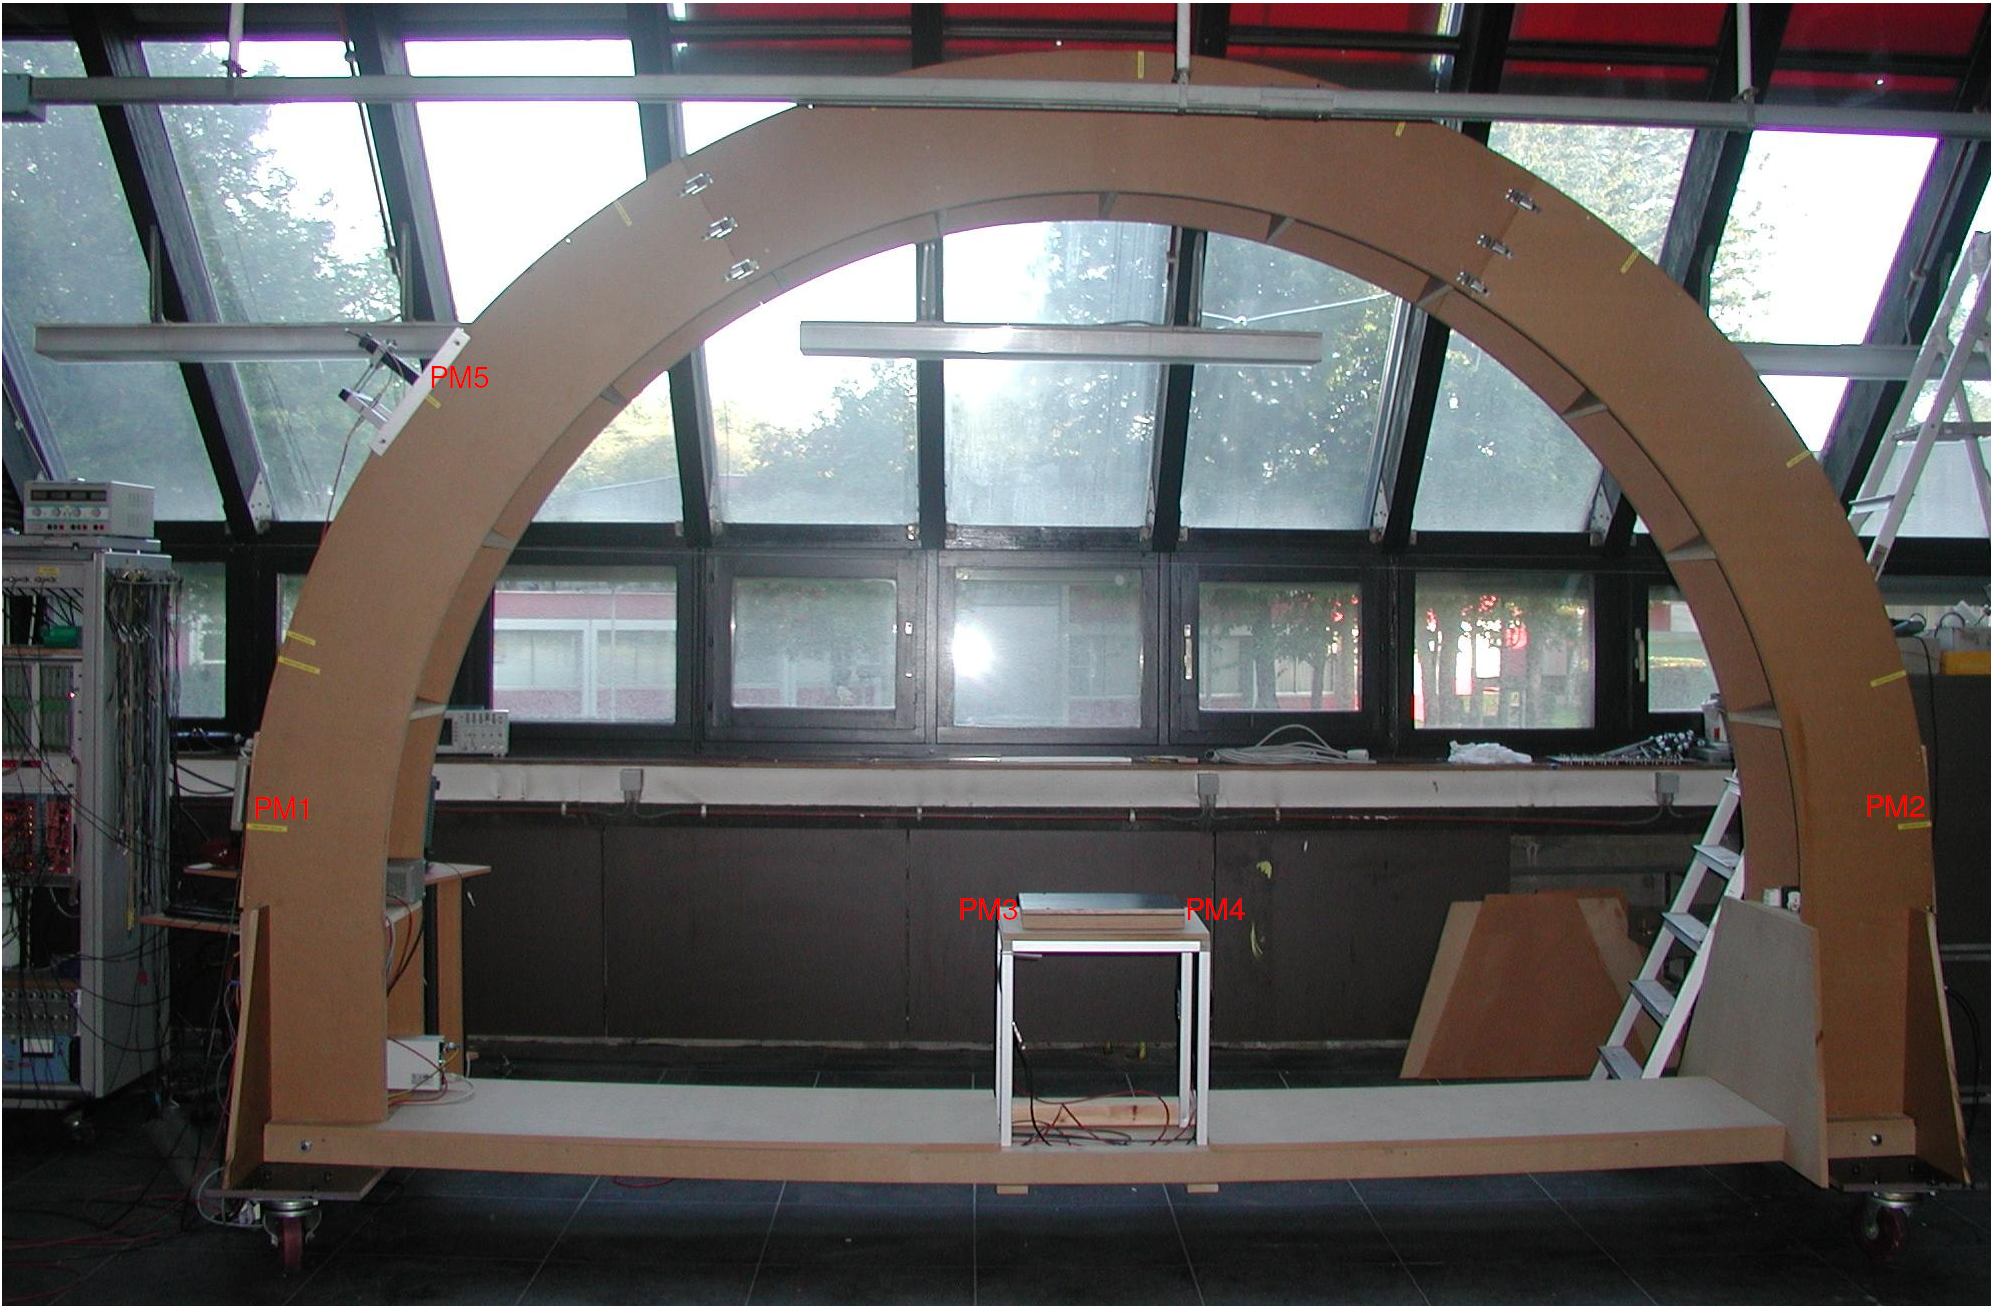
\includegraphics[width=0.75\textwidth]{figures/dispositif_arche.png}
\end{center}
\caption{Photo du dispositif de l'arche précisant la localisation des photomultiplicateurs}
\label{fig:dispositif_arche}
\end{figure}

L'arche, dont la photo est visible sur la figure~\ref{fig:dispositif_arche}, est constituée d'un demi cercle recouvert de blocs scintillants.
Plusieurs guides de lumière (ou \textit{wavelength shifter}) transmettent la lumière produites par scintillation jusqu'aux photomultiplicateurs situés aux pieds de l'arche (PM1\&PM2).
Au centre de celle-ci est installé un autre scintillateur lu par deux photomultiplicateurs (PM3\&PM4).
Ces quatre photomultiplicateurs permettent de sélectionner des muons passant à la fois par le plan et le centre de l'arche.
En mesurant la différence de temps entre l'arrivée des signaux sur les PM1\&PM2, il est possible d'extraire l'angle d'incidence du muon détecté.
Un cinquième scintillateur accompagné de son photomultiplicateur (PM5) ainsi que des LEDs installées le long de l'arche complètent le dispositif à des fins de calibration.

Les dimensions, qui vous aideront lors de l'analyse des données, sont les suivantes:
\begin{itemize}
    \item Dimension des scintillateurs PM3, PM4 \& PM5: \(\SI{21}{\cm}\textrm{ x }\SI{21}{\cm}\)
    \item Largeur des blocs scintillants sur l'arche: \(\SI{21}{\cm}\)
    \item Longueur des blocs scintillants sur l'arche: \(\SI{517}{\cm}\)
    \item Rayon de l'arche: \(\SI{398.3}{\cm}\)
\end{itemize}

\subsection{Prise de mesures}
L'expérience aura été préalablement préparée de sorte à ce que le matériel soit fonctionnel à proximité immédiate.
Afin de vous familiarisez avec le dispositif et de lancer l'acquisition des données, il vous est demandé de suivre les étapes suivantes:

\begin{center}
\fbox{
\begin{minipage}{0.75\textwidth}
    \textbf{Se familiariser avec le dispositif :} 
    \begin{itemize}
        \item Vérifier le signal des différents PMs
        \item Étudier l'efficacité d'un PM
        \item Mesurer l'efficacité angulaire de l'arche
        \item Mesurer la relation entre la position et la différence de temps
        \item Préparer la prise de données
    \end{itemize}
\end{minipage}
}
\end{center}

\subsubsection{Mise en route du dispositif}

Après avoir mis sous tension les PMs, essayez d'observer des signaux sur chacun d'entre eux à l'aide de l'oscilloscope.
Correspondent-il à ce à quoi vous vous attendez ?
Essayez d'observer des coincidences.
Une fois le fonctionnement des PMs établi, utilisez les discriminateurs pour convertir les signaux analogiques en signaux numériques.

\textit{Pour gagner du temps, vous pouvez régler immédiatement la tension du PM5 sur \(\SI{1300}{V}\) et le seuil de son discriminateur sur \(\SI{-80}{\mV}\).}

\paragraph{Attention} Veillez à ne pas dépasser la tension de \(\SI{900}{V}\) sur les PM3\&PM4 pour de pas les endommager.

\subsubsection{Mesure d'efficacité}
Afin de mieux comprendre le comportement des PMs et de les régler au mieux, vous devez mesurer leur efficacité en fonction de la tension d'alimentation et du seuil du discriminateur.
Cette opération se déroule en deux étapes.
Dans un premier temps, faites varier le seuil du discriminateur jusqu'à atteindre le plateau d'efficacité.
Une fois le seuil idéal sélectionné, répétez l'opération, mais en faisant varier la tension cette fois.
Si vous avez suffisamment de temps, il vous est possible de répéter la première mesure pour la nouvelle tension d'alimentation.

De quels PMs allez-vous mesurer l'efficacité ?
Comment allez-vous utiliser la logique NIM ?
N'oubliez pas de mesurer le taux d'événements détectés par le PM en cours de test.

\ifthenelse{\boolean{showAdditional}}{
\begin{additional}
    La mesure de l'efficacité du PM5 est rendue délicate par la présence de fausses coincidences entre les PM3\&PM4.
    Dans le cadre de se laboratoire, il est préférable de mesurer les efficacités des PM3\&PM4 (simultanément si besoin pour gagner du temps).

    \bigskip

    Les opérations logiques à implémenter sont les suivantes:
    \begin{itemize}
        \item Output 1: PM3\&PM5
        \item Output 2: PM4\&PM5
        \item Output 3: PM3\&PM4\&PM5 (attention, cette condition implique les deux conditions précédentes)
    \end{itemize}

    \bigskip

    Ces signaux, ainsi que les signaux en sortie des discriminateurs, doivent être comptés grâce au \textit{scaler}.

    % \begin{figure}
    % \begin{center}
    %     \includegraphics{figures/arche_pm3_pm4.png}
    % \end{center}
    % \caption{Caractérisation de PM3\&PM4 de l'arche}
    % \label{fig:arche_pm3_pm4}
    % \end{figure}
\end{additional}
}

\subsubsection{Mesure de l'efficacité angulaire}

Cette expérience est basée sur le comptage d'événements fonction de l'angle d'incidence des muons atmosphériques.
En conséquence, toute différence d'efficacité dépendante de l'angle doit être corrigée.

Maintenant que les seuils de fonctionnement pour les PM3, PM4 \& PM5 sont établis, vous allez devoir:
\begin{enumerate}
    \item Trouver les seuils optimaux pour les PM1\&PM2 en suivant la procédure utilisée précédemment. \textit{Les tensions d'alimentation ne sont pas réglables.}
    \item Mesurer l'efficacité des PM1\&PM2 pour différents angles d'incidence. Calculer l'efficacité angulaire totale.
\end{enumerate}

Mesurez-vous l'efficacité angulaire de manière optimale ?
Comment utilisez-vous cette information dans votre analyse ?

\ifthenelse{\boolean{showAdditional}}{
\begin{additional}
    La mesure d'efficacité angulaire n'est pas optimale dans notre cas.
    Par manque de temps, la mesure d'efficacité est effectuée en utilisant tous les angles d'incidence alors que la mesure finale n'utilise que les muons normaux à l'arche. 

    En fonction de la manière d'analyser les données, la correction est plus ou moins facile à appliquer.
    Si les données sont mises en boite, il suffit de donner un poids égal à l'inverse de l'efficacité pour chaque événement.
    Si les données ne sont pas mises en boîte, la fonction à ajuster doit être multipliée par l'efficacité point par point.

    D'habitude les résultats ne sont pas nettement améliorés lorsque la correction est appliquée.
    Implémenter cette correction ne devrait se faire que si le temps le permet.

    \begin{center}
        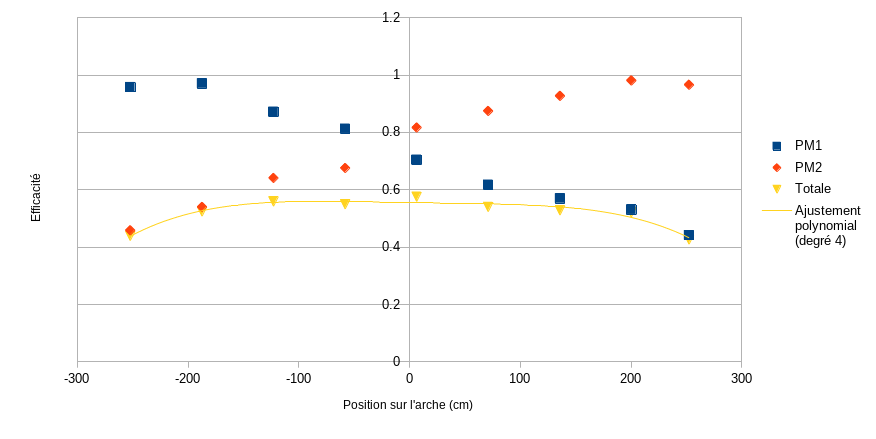
\includegraphics[width=0.7\textwidth]{figures/arche_eff_angulaire.png}
        \\ Efficacité en fonction de l'angle zénithal
    \end{center}
\end{additional}
}

\subsubsection{Calibration de la position en fonction de la différence de temps}

La dernière étape avant la prise de donnée consiste en la mesure de la relation entre la différence de temps d'arrivée des signaux des PM1\&PM2 et la position le long de l'arche.
À cette fin, 15 LEDs ont été insérées dans les blocs scintillants placés le long de l'arche.
Les modules NIM présents vous permettent de pulser individuellement chacune des LEDs.
Le module TDC VME permet de mesurer des temps avec une résolution de \(\SI{25}{\ps}\) dans une fenêtre réglable autour d'un signal de déclenchement (\textit{trigger})\footnote{Plus de documentation sur les réglages de ce modèle de TDC vous est fournie durant le laboratoire.}.

Comment allez-vous faire pulser les LEDs?
Comment réglez-vous la fenêtre d'acquisition du TDC?
Quel \textit{trigger} utilisez-vous?

\ifthenelse{\boolean{showAdditional}}{
\begin{additional}
    En utilisant les deux unités du module \textit{dual-timer}, il est possible de générer un signal de période et de rapport cyclique voulus.
    Pour se faire, il faut connecter la sortie \textit{end-marker} à l'entrée \textit{start} pour chacune des deux unités.
    Les caractéristiques du signal se vérifient facilement à l'oscilloscope.
    Attention à utiliser une fréquence de pulsation suffisamment basse afin de ne pas saturer la lecture du TDC !

    Le \textit{trigger} idéal est dans ce cas ci le signal de commande des LEDs.
    La fenêtre est établie en visualisant les signaux à l'oscilloscope.

    % \begin{figure}
    % \begin{center}
    %     \includegraphics{figures/arche_tdc_led4.png}
    % \end{center}
    % \caption{Exemple de distribution temporelle pour la LED4}
    % \label{fig:arche_tdc_led4}
    % \end{figure}

    % \begin{figure}
    % \begin{center}
    %     \includegraphics{figures/arche_vitesse_lumiere.png}
    % \end{center}
    % \caption{Position sur l'arche en fonction de la différence de temps mesurée}
    % \label{fig:arche_vitesse_lumière}
    % \end{figure}
\end{additional}
}

\subsubsection{Prise de données}

La prise de données constitue la dernière étape de la manipulation.
Pour cela vous devrez définir la logique d'acquisition et l'implémenter les modules NIM et VME.
Celle-ci est similaire à la logique que vous avez développée au point précédent: il vous faut mesurer la différence de temps d'arrivée des signaux des PM1\&PM2.
Dans ce cas ci, nous nous intéressons à des muons atmosphériques qui passent simultanément par le plan et le centre de l'arche. Pourquoi ?

Quelle logique allez-vous implémenter ?
Quels réglages utilisez-vous pour le TDC ?

\ifthenelse{\boolean{showAdditional}}{
\begin{additional}
    La logique fournissant le \textit{trigger} est une coincidence entre les PM1\&PM2\&PM3(4)\&PM5.
    Ainsi, on est assuré de sélectionner des muons étant passés, et ayant été mesurés, à la fois par le plan et le centre de l'arche.
    Cette configuration est évidente pour mesurer un angle zénithal, on peut voir l'arche comme un rapporteur géant.

    Pour ne pas perdre d'événements, il faut faire particulièrement attention à deux points:
    \begin{enumerate}
        \item Les signaux doivent être correctement mis en temps.
              Ceci est complexifié par le fait que les temps d'arrivée des PM1\&PM2 varient événement par événement.
              Les largeurs des fenêtres en sortie des discriminateurs doivent donc être suffisamment grandes.
        \item La fenêtre d'acquisition du TDC doit être correctement configurée.
              Observer les signaux de tous les PMs se révèle être une aide précieuse dans cet objectif.
    \end{enumerate}

    % \begin{figure}
    % \begin{center}
    %     \includegraphics{figures/arche_distribution.png}
    % \end{center}
    % \caption{Distribution des différences de temps mesurées (aucune correction appliquée)}
    % \label{fig:arche_distribution.png}
    % \end{figure}
\end{additional}
}

\subsection{Analyse des données}

A présent, nous pouvons nous concentrer sur l'analyse des données afin de vérifier la loi en \(\cos^2(\theta)\).
En vous basant sur l'ensemble de vos données, il vous est demandé de calculer:

\begin{center}
\fbox{
\begin{minipage}{0.75\textwidth}
    \textbf{Arche cosmique :}
    \begin{itemize}
        \item La vitesse de la lumière dans le guide de lumière
        \item La puissance \(\alpha\) et l'alignement \(\theta_0\) dans la loi \(\cos^{\alpha}(\theta-\theta_0)\)
    \end{itemize}
\end{minipage}
}
\end{center}


\end{document}
